\documentclass{diploma}

\usepackage{siunitx}

\student{Бирюков Виктор Владимирович}
\group{М8О-407Б-19}
\theme{Разреженная идентификация нелинейных динамических систем}

\supervisor{Ревизников Дмитрий Леонидович}
\firstConsultant{---}
\secondConsultant{---}
\reviewer{---}

\faculty{№ 8 <<Компьютерные науки и прикладная математика>>}
\department{806}
\speciality{01.03.02 <<Прикладная математика и информатика>>}
\profile{Информатика}

\departmentFullName{№ 806}
\headOfDepartment{Крылов Сергей Сергеевич}
\date{\uline{\hspace{24pt}} мая \the\year\ года}

% \newacronym{sindy}{SINDy}{sparse identification of nonlinear dynamics}
% \newacronym{lasso}{Lasso}{least absolute shrinkage and selection operator}
% \newacronym{stlsq}{STLSQ}{sequential thresholded least-squares}
% \newacronym{мнк}{МНК}{метод наименьших квадратов}
% \newacronym{tvr}{TVR}{total variation regularization}
% \newacronym{оду}{ОДУ}{обыкновенное дифференциальное уравнение}
% \newacronym{слау}{СЛАУ}{система линейных алгебраических уравнений}
% \newacronym{iou}{IoU}{intersection over union}

\newglossaryentry{iou}{name={IoU}, description={intersection over union}}
\newglossaryentry{lasso}{name={Lasso}, description={least absolute shrinkage and selection operator}}
\newglossaryentry{sindy}{name={SINDy}, description={sparse identification of nonlinear dynamics}}
\newglossaryentry{stlsq}{name={STLSQ}, description={sequential thresholded least-squares}}
\newglossaryentry{tvr}{name={TVR}, description={total variation regularization}}
\newglossaryentry{мнк}{name={МНК}, description={метод наименьших квадратов}}
\newglossaryentry{оду}{name={ОДУ}, description={обыкновенное дифференциальное уравнение}}
\newglossaryentry{слау}{name={СЛАУ}, description={система линейных алгебраических уравнений}}
\newglossaryentry{id1}{
    name={Уровень шума},
    description={дисперсия белого гауссова шума с нулевым математическим ожиданием} 
}

\addbibresource{main.bib}

\graphicspath{ {./img/} }

% Иллюстрации всегда по центру
\makeatletter
\g@addto@macro\@floatboxreset\centering
\makeatother

\begin{document}
    \maketitle

    % \includepdf[pages=-]{extra/task}
    \setcounter{page}{2} % Устанавливает счётчик страниц

    \abstract

\keywords{ДИНАМИЧЕСКИЕ СИСТЕМЫ, ИДЕНТИФИКАЦИЯ СИСТЕМ, РАЗРЕЖЕННАЯ РЕГРЕССИЯ, ЧИСЛЕННОЕ ДИФФЕРЕНЦИРОВАНИЕ, ОБЫКНОВЕННЫЕ ДИФФЕРЕНЦИАЛЬНЫЕ УРАВНЕНИЯ}

Объектом исследования в данной работе являются нелинейные динамические системы.

Цель работы –-- идентификация систем обыкновенных дифференциальных уравнений первого порядка на основе потенциально шумных данных.

Для достижения поставленной цели были проведены исследования в области алгоритмов идентификации, а также разреженной регрессии и численного дифференцирования.

Основное содержание работы состояло в разработке алгоритма идентификации и его составных частей: алгоритмов разреженной регрессии и устойчивого численного дифференцирования.

Основными результатами работы, полученными в процессе разработки, являются алгоритм идентификации, рекомендации по его использованию, а также рекомендации по использованию методов дифференцирования, которые для данной задачи используются впервые.

Результаты разработки предназначены для извлечения математических закономерностей из данных --- структурного анализа.

Использование результатов данной работы позволяет существенно расширить возможности анализа данных, так как появляется возможность использовать соответствующий математический аппарат для анализа самой системы.

    \tableofcontents
    \termsandabbreviations

    \introduction

Актуальность темы данной работы связана с распространенностью нелинейных динамических систем для описания различных процессов. В случаях, когда существуют только дискретные данные, собранные, например, в результате эксперимента, возникает задача по идентификации системы, лежащей за этими данными. Такая задача может осложняться большим объемом данных, их сложностью или наличием в них посторонних шумов, что делает проблематичным ее решение в ручном режиме.

Таким образом, выполненная работа актуальна и с теоретической, и с практической точек зрения.

Цель работы --– идентификация систем обыкновенных дифференциальных уравнений первого порядка на основе потенциально шумных данных.

Для достижения поставленной цели в работе были решены следующие задачи:
\begin{itemize}
  \item реализация алгоритма идентификации;
  \item реализация алгоритмов дифференцирования шумных данных;
  \item реализация алгоритмов разреженной регрессии;
  \item тестирование алгоритма идентификации на известных системах ОДУ 1-ого порядка;
  \item сравнение различных методов дифференцирования и регрессии.
\end{itemize}

Работа основывалась на следующих инструментах и методах:
\begin{itemize}
  \item язык программирования Python,
  \item библиотеки научных вычислений NumPy и SciPy,
  \item библиотека машинного обучения Scikit-learn,
  \item библиотеки построения графиков Matplotlib и Seaborn,
  \item среда разработки Jupyter.
\end{itemize}

Основными результатами, полученными в работе, являются:
\begin{itemize}
\item работающий алгоритм идентификации систем ОДУ по шумным данным;
\item рекомендации по использованию алгоритма идентификации;
\item реализация алгоритмов численного дифференцирования методом регуляризации полной вариации;
\item рекомендации по подбору параметров и использованию алгоритмов дифференцирования.
\end{itemize}

Результаты работы предназначены для использования в анализе данных.

Использование разработки позволяет выявлять в данных закономерности, которые могут быть описаны при помощи нелинейных динамических систем различного вида, например, систем ОДУ 1-ого порядка. Это существенно расширяет возможности анализа данных, так как позволяет использовать соответствующий математический аппарат для анализа самой системы.


    \section{ПОСТАНОВКА ЗАДАЧИ}

\subsection{Актуальность работы}

Извлечение математических закономерностей из данных --- структурный анализ --- является важной задачей во многих научных областях. Существует много проблем, связанных с данными, таких как понимание когнитивных процессов на основе мозговой активности, изучение закономерностей климата, определение устойчивости финансовых рынков, прогнозирование и подавление распространения болезней. В связи с обилием данных, роль структурного анализа в этих сферах вероятно будет только расти.

Достижения в области машинного обучения и науке о данных привели к продвижению в анализе и понимании сложных данных, извлечение закономерностей из которых превышает возможности человека. Однако, несмотря на быстрое развитие инструментов на основе статистических отношений, замедлился прогресс в извлечении физических моделей динамических процессов. Это приводит к тому, что имеющиеся методы не могут экстраполировать результат за пределы аттрактора, в котором данные были получены.

Поэтому более перспективными кажутся методы, извлекающие закономерности в символьном виде. Первым прорывом в этой области стало использование символьной регрессии и генетического программирования для поиска нелинейных дифференциальных уравнений \cite{symbolic, genetic}. В таком подходе балансируется сложность модели, измеряемая количеством членов, с точностью идентификации. Однако символьная регрессия вычислительно сложна, а также плохо масштабируется и склонна к переобучению.

Другим методом, который и рассматривается в данной работе, является решение задачи идентификации с точки зрения разреженной регрессии \cite{sindy, lasso}. При этом активно используется тот факт, что большинство физических систем имеют небольшое количество значимых членов, что делает их разреженными в пространстве нелинейных функций. Это позволяет избежать комбинаторного взрыва, который возникает при обычном переборе. В результате процесс идентификации обеспечивает естественное балансирование сложности модели, которая определяется разреженностью правых частей уравнений, с точностью. Использование алгоритмов выпуклой оптимизации позволяет применять метод к задачам большого масштаба.

В таком подходе также можно усмотреть сходство с методом разложения по динамическим модам (dynamic mode decomposition) \cite{dmd}, который является линейной динамической регрессией. Этот метод опирается только на исходные данные, а не на знание уравнений динамики, и также связан с теорией операторов Купмана \cite{koopman}. Однако при использовании этого метода все равно необходимы предположения о виде динамической системы, поскольку на данный момент нет методов по определению наблюдаемых функций. В отличие от этого, использование разреженной регрессии позволяет автоматически определять значимые члены в динамических системах.

\subsection{Техническое задание}

Таким образом, целью работы является реализация алгоритма идентификации нелинейных систем на основе данных.

Входные данные представляют из себя массив замеров некоторых величин, описывающих динамическую систему. Так как алгоритм нацелен на использование с реальными системами и данными, полученными экспериментальным путем, входные данные могут содержать некоторую шумовую компоненту. Поэтому разработанный алгоритм должен быть устойчив к этому шуму.

Задача идентификация ограничивается системами обыкновенных дифференциальных уравнений первого порядка. Системы ОДУ 1-ого порядка позволяют описать довольно много процессов реального мира и для их идентификации достаточно базовой версии алгоритма и производных первого порядка.

В качестве источника данных используются известные системы ОДУ. Данные получаются синтетическим путем.


    \section{РАЗРЕЖЕННАЯ ИДЕНТИФИКАЦИЯ НЕЛИНЕЙНЫХ ДИНАМИЧЕСКИХ СИСТЕМ}

\subsection{Теоретическое описание}

\subsubsection{Структурный анализ нелинейных динамических систем}

Алгоритм, описываемый в данной работе, позволяет производить структурную идентификацию динамических систем \cite{sindy} вида:

\begin{equation}
\dot{\textsc{x}}(t) = f(\textsc{x}(t)),
\end{equation}

где вектор $\textsc{x}(t) = \left(x_1(t) \quad x_2(t) \quad \cdots \quad x_n(t)\right)^T \in \mathbb{R}^n$ описывает состояние системы в момент времени $t$;\par 
$f(\textsc{x}(t))$ --- нелинейная функция, описывающая поведение самой системы.

Ключевое наблюдение, лежащее в основе алгоритма, состоит в том, что большое число таких функций представляют из себя линейную комбинацию небольшого количества значимых членов, другими словами, они являются разреженными в пространстве возможных функций.

Для проведения структурной идентификации необходимо собрать множество измерений состояний системы $\textsc{x}(t)$ и соответствующие им значения производной. Эти измерения образуют две матрицы:

\begin{equation}
X =
\begin{pmatrix}
\textsc{x}^T(t_1) \\	
\textsc{x}^T(t_2) \\
\vdots \\	
\textsc{x}^T(t_m)	
\end{pmatrix}
=
\begin{pmatrix}
x_1(t_1) & x_2(t_1) & \cdots & x_n(t_1) \\
x_1(t_2) & x_2(t_2) & \cdots & x_n(t_2) \\
\vdots & \vdots & \ddots & \vdots \\
x_1(t_m) & x_2(t_m) & \cdots & x_n(t_m)
\end{pmatrix}
\end{equation}

\begin{equation}
\dot{X} = 
\begin{pmatrix}
\dot{\textsc{x}}^T(t_1) \\	
\dot{\textsc{x}}^T(t_2) \\
\vdots \\	
\dot{\textsc{x}}^T(t_m)	
\end{pmatrix}
=
\begin{pmatrix}
\dot{x_1}(t_1) & \dot{x_2}(t_1) & \cdots & \dot{x_n}(t_1) \\
\dot{x_1}(t_2) & \dot{x_2}(t_2) & \cdots & \dot{x_n}(t_2) \\
\vdots & \vdots & \ddots & \vdots \\
\dot{x_1}(t_m) & \dot{x_2}(t_m) & \cdots & \dot{x_n}(t_m)
\end{pmatrix}.
\end{equation}

В случае использования реальных экспериментальных данных (или синтезированных данных, которые призваны их заменить) значения производных будут неизвестны. В связи с этим возникает задача численного дифференцирования для получения данных значений. Такая задача может быть осложнена наличием шума в данных, что требует специальных алгоритмов дифференцирования, способных справиться с подобными затруднениями.

Следующим этапом составляется матрица признаков $\Theta(X)$, которая содержит нелинейные функции от столбцов $X$, предположительно содержащиеся в искомой системе. Например, она может состоять из константной функции, полиномов и тригонометрических функций:

\begin{equation}
\fontsize{13pt}{15pt}\selectfont
\renewcommand*{\arraystretch}{.5}
\Theta(X) = 
\begin{pmatrix}
| & | & | & | &  & | & | & | & | &  \\
1 & X & X^{P_2} & X^{P_3} & \cdots & \sin(X) & \cos(X) & \sin(2X) & \cos(2X) & \cdots \\
| & | & | & | &  & | & | & | & | & 
\end{pmatrix},
\end{equation}

где $X^{P_2}$, $X^{P_3}$ обозначают полиномы второй и третьей степени соответственно, например:

\begin{equation}
X^{P_2} = 
\begin{pmatrix}
x_1^2(t_1) & x_1(t_1) x_2(t_1) & \cdots & x_2^2(t_1) & x_2(t_1) x_3(t_1) & \cdots & x_n^2(t_1) \\ 
x_1^2(t_2) & x_1(t_2) x_2(t_2) & \cdots & x_2^2(t_2) & x_2(t_2) x_3(t_2) & \cdots & x_n^2(t_2) \\
\vdots & \vdots & \ddots & \vdots & \vdots & \ddots & \vdots \\
x_1^2(t_m) & x_1(t_m) x_2(t_m) & \cdots & x_2^2(t_m) & x_2(t_m) x_3(t_m) & \cdots & x_n^2(t_m)
\end{pmatrix}.
\end{equation}

Теперь задача заключается в определении того, как именно надо скомбинировать столбцы матрицы признаков для получения векторов левых частей. Это есть ни что иное, как задача линейной регрессии, при этом, так как было сделано предположение, что искомая функция содержит небольшое число значимых членов, это конкретный подвид линейной регрессии --- разреженная регрессия --- при помощи которого можно получить разреженную матрицу коэффициентов $W$:

\begin{equation}
\dot{X} = \Theta(X) W.
\end{equation}

Столбцы матрицы $W$ определяют значимые члены правых частей каждого из уравнений системы и коэффициенты перед ними.

Таким образом, основными частями алгоритма являются численное дифференцирование и разреженная регрессия. Рассмотрим каждую из них подробно.


    \subsubsection{Разреженная регрессия}

Задача линейной регрессии формулируется следующим образом. Имеется множество объектов и множество соответствующих им значений целевой переменной. Необходимо подобрать такие коэффициенты линейной комбинации признаков объектов, чтобы она лучше всего приближала значения целевой переменной в смысле некоторой функции потерь (обычно среднеквадратичного отклонения).

Таким образом, пусть имеется вектор значений целевой переменной $y = (y_i)_{i=1}^N \in \mathbb{R}_N$ и матрица признаков $X = (x_i)_{i=1}^N \in \mathbb{R}^{N \times D}$, $x_i \in \mathbb{R}^D$. Функция потерь имеет вид:

\begin{equation}
L(w) = \frac{1}{N} ||y - X w||^2_2 \longrightarrow \min_w,
\end{equation}

где $w$ --- искомые веса.

К решению такой задачи существует несколько подходов. Во-первых, можно получить аналитическое решение. Действительно, градиент функции потерь имеет вид:

\begin{equation}
\nabla L = \frac{2}{N} X^T (X w - y),
\end{equation}

а вторая производная:

\begin{equation}
L'' = \frac{2}{N} X^T X.
\end{equation}

Функция потерь квадратичная, следовательно имеет один экстремум, который является точкой минимума, так как матрица $\frac{2}{N} X^T X$ положительно определена (для любого $X$ с линейно независимыми столбцами). Таким образом, по необходимому условию экстремума, искомое $w$ получается как решение матричного уравнения:

\begin{align}
&X^T (X w - y) = 0 \\
&w = (X^T X)^{-1} X^T y.
\end{align}

Такое решение будет точным, однако, его вычисление включает в себя операцию обращения матрицы, что вычислительно дорого и может быть неприемлемо для большого объема данных. Более того, можно столкнутся с проблемой плохой обусловленности матрицы, что приведет к неустойчивости решения.

Поэтому другой способ заключается в решении задачи оптимизации методом градиентного спуска. Зная градиент функции потерь, само решение можно вычислить следующим итеративным процессом:

\begin{equation}
w_{k+1} = w_k - \eta \cdot \nabla L(w_k), 
\end{equation}

где $\eta$ --- скорость обучения --- контролирует величину шага в направлении антиградиента.

При помощи этого метода можно получать решение с некоторой точностью, но со значительно меньшим использованием вычислительных ресурсов.

Проблема описанного выше подхода (для любого метода решения) заключается в том, что на веса не накладывается никаких дополнительных ограничений. Это может привести, например, к их неограниченному росту при наличии коррелированных признаков, но, что более важно, каждому признаку будет приписан какой-то ненулевой вклад в целевую функцию. Этот вклад может быть очень маленьким, но его наличие не позволяет, например, просто откинуть наименее важные признаки, так как это потребует пересчета оставшихся весов и незначимые признаки могут возникнуть вновь.

Поэтому возникает потребность в алгоритмах разреженной регрессии, частью которых является отбор признаков и по результатам которых можно точно отделить признаки, не вносящие вклада в целевую функцию.

\paragraph{Lasso}

Одним из способов решения задачи разреженной регрессии является использование регуляризации --- штрафа на величину весов, который добавляется в функцию потерь. Наиболее распространены $L_1$ и $L_2$ регуляризации, в которых штраф имеет вид $L_1$ нормы $||w||_1 = \sum_i |w_i|$ и $L_2$ нормы $||w||_2 = \sqrt{\sum_i |w_i|^2}$ весов соответственно. В отличие от $L_2$ регуляризации, которая приводит только к уменьшению величины весов, $L_1$ регуляризация позволяет обнулять коэффициенты при самых незначимых признаках. В результате получается алгоритм Lasso --- Least absolute shrinkage and selection operator \cite{lasso}.

Вместе с добавленным штрафом, функция потерь выглядит следующим образом:

\begin{equation}
L(w) = \frac{1}{N} ||y - X w||^2_2 + \alpha ||w||_1,
\end{equation}

где $\alpha$ --- коэффициент регуляризации.

Технически, $L_1$ норма недифференцируема. Однако недифференцируема она только в одной точке (в нуле). Применительно к машинному обучению, можно считать, что вероятность встречи точного нуля крайне мала, и пренебречь этим. Тогда производная $L_1$ нормы --- это знаковая функция $\operatorname{sign}$, доопределенная в нуле (при помощи $1$ или $-1$). Таким образом градиент функции потерь:

\begin{equation}
\nabla L(w) = \frac{2}{N} X^T (X w - y) + \alpha \operatorname{sign}(w).
\end{equation}

Для получения решения используем метод градиентного спуска.

\paragraph{STLSQ}

Помимо классического Lasso авторы алгоритма идентификации предлагают собственный алгоритм разреженной регрессии STLSQ --- Sequential Thresholded Least-Squares \cite{sindy}.

Алгоритм заключается в следующем. Найдем решение задачи регрессии при помощи МНК --- метода наименьших квадратов --- любым способом. Такое решение не будет разреженным, но некоторые коэффициенты в нем будут меньше других. Обнулим коэффициенты, меньшие некоторого порогового значения $\alpha$. После этого снова найдем решение МНК, но уже для оставшихся коэффициентов, и опять обнулим коэффициенты. Эта процедура уточнения и отбора коэффициенты повторяется, пока все ненулевые не станут больше $\alpha$. Если произошло обнуление вообще всех коэффициентов, значит порог $\alpha$ выбран слишком большим и его надо уменьшить. Псевдокод алгоритма представлен на рисунке~\ref{alg:stlsq}.

\begin{figure}
\begin{minipage}{\linewidth}
\begin{algorithm}[H]
\SetAlgoVlined
\KwData{пороговое значение $\alpha$}
\KwIn{матрица признаков $X$, вектор целевой переменной $y$}
\KwOut{вектор весов $w$}

$w = \operatorname{solve}(X, y)$ \tcp*[l]{функция solve использует МНК}
\While{вектор $w$ изменяется}{
	$smallinds = |w| < \alpha$\;
	$w[smallinds] = 0$\;

	$biginds = \neg smallinds$\;
	$w[biginds] = \operatorname{solve}(X[biginds], y)$\;
}
\end{algorithm}
\end{minipage}
\caption{Псевдокод алгоритма STLSQ}
\label{alg:stlsq}
\end{figure}

Приведенные выше алгоритмы описаны для одной целевой функции, однако, они легко обобщаются на случай нескольких целевых функций. Lasso, как и другие алгоритмы, основанные на градиентном спуске, практически не требует изменений, так как градиент можно вычислять для любой размерности. В случае STLSQ алгоритм надо выполнять отдельно для каждого вектора целевых функций и весов.
    \subsubsection{Численное дифференцирование}

\paragraph{Конечно-разностный метод}

Простейшими методами численного дифференцирования является семейство методов, использующих конечные разности. В таких методах оператор дифференцирования аппроксимируется отношением конечных разностей, которое получается путем дифференцирования аппроксимирующего многочлена. Используя многочлены различных степеней, можно получить конечно-разностные формулы соответствующего порядка аппроксимации.

Пусть функция $f(x)$ задана таблично $f_i = f(t_i),\ i = \overline{1, n}$ на регулярной сетке с шагом $x_{i+1} - x_i = h$. Тогда для вычисления производной первого порядка в тех же точках $f'_i = f'(t_i),\ i = \overline{1, n}$ будем использовать следующие конечно-разностные формулы:

\begin{align}
f'_1 &= \frac{-3 f_1 + 4 f_2 - f_3}{2 h} \\
f'_i &= \frac{f_{i+1} - f_{i-1}}{2 h}, \qquad i = \overline{2, n-1} \\
f'_n &= \frac{f_{n-2} - 4 f_{n-1} + 3 f_n}{2 h}.
\end{align}

Такие формулы обеспечивают второй порядок аппроксимации.

Значительным недостатком конечно-разностного метода является то, что при наличии шумовой составляющей в используемых данных $x_i$, шумовая составляющая усиливается, что приводит к некорректным значениям производной. Таким образом, с точки зрения практического использования этот метод имеет очень узкую область применимости.

\paragraph{Регуляризация полной вариации}

Более устойчивый к шуму метод можно получить, используя регуляризацию самого процесса дифференцирования, а именно --- регуляризацию полной вариации.

Полная вариация является обобщением понятия длины кривой, задаваемой произвольной функцией $f: [a, b] \rightarrow \mathbb{R}^n$. Если $f \in C^1$, то есть имеет непрерывную первую производную, $f$ является функцией ограниченной вариации, которая вычисляется по формуле:

\begin{equation}
\int\limits_a^b ||f'(x)||\,\mathrm{d}(x),
\end{equation}

где $||\cdot||$ --- некоторая норма в пространстве $\mathbb{R}^n$.

Задачу дифференцирования функции $f' = u$ на отрезке $[0, L]$ можно свести к интегральному уравнению Вольтерра первого рода:

\begin{equation}
\int_0^x u(s)\,\mathrm{d}(s) = f(x) - f(0),
\end{equation}

где $x \in [0, L]$.

Обозначим $A u (x) = \int_0^x u$ --- оператор интегрирования, также предположим, что $f(0) = 0$ (на практике это достигается вычитанием $f(0)$ из $f$):

\begin{equation}
A u = f.
\end{equation}

Это уравнение относится к некорректным в силу высокой чувствительности решения к малым возмущениям правой части. Непосредственное решение данного уравнения не имеет смысла. Вместо этого будем решать задачу минимизации функционала:

\begin{equation}
F(u) = DF(A u - f) + \alpha R \longrightarrow \min_u,
\end{equation}

где $DF(A u - f)$ --- компонента, отвечающая за точность решения;
\par $\alpha$ --- коэффициент регуляризации;
\par $R$ --- регуляризационная компонента.

Функционал $DF$ обычно представляет из себя квадрат $L^2$ нормы, $DF = \int_0^L |\cdot|^2$, так как предполагается, что $f$ имеет в своем составе белый гауссов шум. Для шумов с другим распределением необходимо использовать другие функционалы.

С этого момента существует несколько подходов к решение этой задачи, связанных с разными формами регуляризации.

\subparagraph{Первый метод}

Первый способ заключается в регуляризации --- в виде квадрата $L^2$ нормы --- производной функции $f$ \cite{fast_tvr}:

\begin{equation}
R = \int\limits_0^L |f'|^2.
\end{equation}

Таким образом происходит регуляризация полной вариации $f$ и функционал $F$ принимает вид:

\begin{equation}
F(u) = \int\limits_0^L |A u - f|^2 + \alpha \int\limits_0^L |f'|.
\end{equation}

Аппроксимируя операторы интегрирования и дифференцирования, можно переписать задачу в матрично-векторной форме (о конкретном виде дискретных аналогов операторов будет сказано позже):

\begin{equation}
F(u) = ||A u - f||_2^2 + \alpha ||D f||_2^2,
\end{equation}

где $u$ --- искомый вектор производных,\par 
$f$ --- вектор приращений функции,\par 
$A$ --- матричный оператор интегрирования,\par 
$D$ --- матричный оператор дифференцирования,\par 
$||\cdot||_2$ --- евклидова норма вектора.

Минимизируемая функция квадратичная, следовательно задача минимизации может быть решена с использованием необходимого условия экстремума:

\begin{equation}
\nabla F(u) = 0.
\end{equation}

В результате задача сводится к решению системы линейных алгебраических уравнений относительно вектора $u$:

\begin{equation}
B u = b,
\end{equation}

где $B = A^T A + \alpha D^T D$,\par $b = A^T u$.

\subparagraph{Второй метод}

Для второго способа вместо квадрата $L^2$ нормы используем $H^1_1$ норму искомой производной $u$ \cite{tvr}:

\begin{equation}
R = \int\limits_0^L |u'|.
\end{equation}

Тогда регуляризации подвергается полная вариация $u$ и функционал $F$ имеет вид:

\begin{equation}
F(u) = \int\limits_0^L |A u - f|^2 + \alpha \int\limits_0^L |u'|.
\end{equation}

Такую задачу минимизации уже нельзя решить, используя только необходимое условие экстремума, и необходимо применять другие методы оптимизации. Простейшим способом будет использовать метод градиентного спуска. Для такой задачи этот метод сводится к эволюции дифференциального уравнения до стационарного состояния:

\begin{equation}
u_t = \alpha \frac{\mathrm{d}}{\mathrm{d}x} \frac{u'}{|u'|} - A^T (A u - f),
\end{equation}

где $A^T v(x) = \int_x^L v$ --- сопряженный оператор к $A$.

Во избежании деления на ноль, $|u'|$ в знаменателе можно заменить на $\sqrt{(u')^2 + \varepsilon}$, для некоторого малого $\varepsilon > 0$.

Проблема градиентного спуска состоит в медленной сходимости. Поэтому вместо него предлагается использовать метод запаздывающей диффузии (lagged diffusivity) \cite{lagged_diff_1, lagged_diff_2}. Основная идея этого метода заключается в замене нелинейного дифференциального оператора $u \mapsto (\mathrm{d} / \mathrm{d}x)(u'/|u'|)$ линейным оператором $u \mapsto (\mathrm{d} / \mathrm{d}x)(u'/|u'_k|)$.

Для этого необходимо произвести дискретизацию. Предполагаем, что функция $f$ задана на регулярной сетке с шагом $h$ в точках $\{x_i\}_0^n = \{0, h, 2h, \ldots, L\}$, ее производную $u$ будем искать в точках $\{x_i\}_0^n \cup \{x_{-1}\} = \{-h, 0, h, 2h, \ldots, L\}$ (первая точка нужна только для работы алгоритма и в результат не входит). Производную $u$ будем вычислять между точками сетки, как центральные разности:

\begin{equation}
D u(x_i + \frac{h}{2}) = \frac{u(x_{i+1} - u(x_i))}{h}, \qquad i = \overline{-1, n-1}. 
\end{equation}

Интеграл от $u$ будем вычислять в точках $\{x_i\}_0^n$, используя метод трапеций:

\begin{equation}
A u(x_i) = \displaystyle\sum_{j=-1}^{i-1} \frac{u(x_j) + u(x_{j+1})}{2} h, \qquad i = \overline{0, n}.
\end{equation}

Таким образом, матрицы операторов интегрирования и дифференцирования, обе размером $n \times (n + 1)$, выглядят следующим образом:   

\begin{equation}
D_{n, n+1} = \frac{1}{h}
\begin{pmatrix}
-1 &  1 &  0 & 0 & \cdots &  0 &  0 &  0 \\
 0 & -1 &  1 & 0 & \cdots &  0 &  0 &  0 \\
 0 &  0 & -1 & 1 & \cdots &  0 &  0 &  0 \\
\vdots & \vdots & \vdots & \vdots & \ddots & \vdots & \vdots & \vdots \\
 0 &  0 &  0 & 0 & \cdots & -1 &  1 &  0 \\
 0 &  0 &  0 & 0 & \cdots &  0 & -1 &  1 
\end{pmatrix}
\end{equation}

\begin{equation}
A_{n, n+1} = h
\begin{pmatrix}
0.5 & 0.5 &   0 &   0 & \cdots & 0 &   0 &   0 \\
0.5 &   1 & 0.5 &   0 & \cdots & 0 &   0 &   0 \\
0.5 &   1 &   1 & 0.5 & \cdots & 0 &   0 &   0 \\
\vdots & \vdots & \vdots & \vdots & \ddots & \vdots & \vdots & \vdots \\
0.5 &   1 &   1 &   1 & \cdots & 1 & 0.5 &   0 \\
0.5 &   1 &   1 &   1 & \cdots & 1 &   1 & 0.5 
\end{pmatrix}.
\end{equation}

Подобные матрицы и подход с дополнительной точкой можно также использовать и в первом методе.

Метод запаздывающей диффузии представляет из себя итеративный процесс. На каждой итерации $k$ используются следующие матрицы:

\begin{align}
E_k &= \operatorname{diag}(((D u_k)^2 + \varepsilon)^{-1/2}),\\
L_k &= h D^T E_k D,\\
H_k &= A^T A + \alpha L_k,
\end{align}

где $\operatorname{diag}(v)$ --- диагональная матрица со значениями вектора $v$ на главной диагонали;\par
$H_k$ --- аппроксимация гессиана $F$ в точке $u_k$.

Переход к следующей итерации:

\begin{align}
& g_k = A^T (A u_k - f) + \alpha L_k u_k, \\
\label{eq:s}
& H_k s_k = g_k, \\
& u_{k+1} = u_k + s_k,
\end{align}

где $s_k$ --- решение системы линейных алгебраических уравнений~(\ref{eq:s}).

Начальным значением $u$ может быть нулевой вектор или вектор производных, полученных методом конечных разностей.
Завершение итеративного процесса можно произвести по достижению заданного числа итераций, или при незначительном изменении вектора $u_k$, относительно предыдущего значения. Псевдокод алгоритма представлен на рисунке~\ref{alg:tvr}.

\begin{figure}
\begin{minipage}{\linewidth}
\begin{algorithm}[H]
\SetAlgoVlined
\KwData{коэффициент регуляризации $\alpha$, число итераций $K$}
\KwIn{вектор значений функции $f$, шаг регулярной сетки $h$}
\KwOut{вектор производных $u$}

$n = \text{размер вектора}\ f$\;
$u = {\underbrace{(0 \ 0 \ \cdots \ 0)}_{n+1}}^T$\;
\For{$k = 1$ \KwTo $K$}{
    $E = \operatorname{diag}(((D u)^2 + \varepsilon)^{-1/2})$\;
    $L = h D^T E D$\;
    $H = A^T A + \alpha L$\;
    $g = A^T (A u - f) + \alpha L u$\;
    $s = \operatorname{solve}(H, g)$ \tcp*[l]{функция solve решает СЛАУ}
    $u = u + s$\;
}
\KwRet{$(u_1 \ u_2 \ \cdots \ u_{n+1})^T$}
\end{algorithm}
\end{minipage}
\caption{Псевдокод второго метода алгоритма дифференцирования}
\label{alg:tvr}
\end{figure}

    \subsection{Используемые технологии}

Основной и единственный язык реализации --- Python \cite{python}. Это очень удобный язык программирования для работы с данными и реализации алгоритмов машинным обучением.

Так как большинство алгоритмов реализовывались полностью с нуля, в них активно используются две основные библиотеки научных вычислений --- NumPy \cite{numpy} и SciPy \cite{scipy}.

При разработке использовался объектно-ориентированный подход на основе базовых классов библиотеки Scikit-learn \cite{sklearn}. Эта библиотека предоставляет крайне удобную инфраструктуру для алгоритмов машинного обучения.

При тестировании и анализе методов использовалась среда разработки Jupyter \cite{jupyter}.

Для визуализации использовались библиотеки Matplotlib \cite{matplotlib} и Seaborn~\cite{seaborn}.

    \subsection{Описание программной разработки}
\label{section:practice}

Разработанное решение реализовано в формате модуля языка Python. Структура модуля изображена на рисунке~\ref{fig:tree}, служебные файлы (такие как \texttt{\_\_init\_\_.py}) опущены.

\begin{figure}
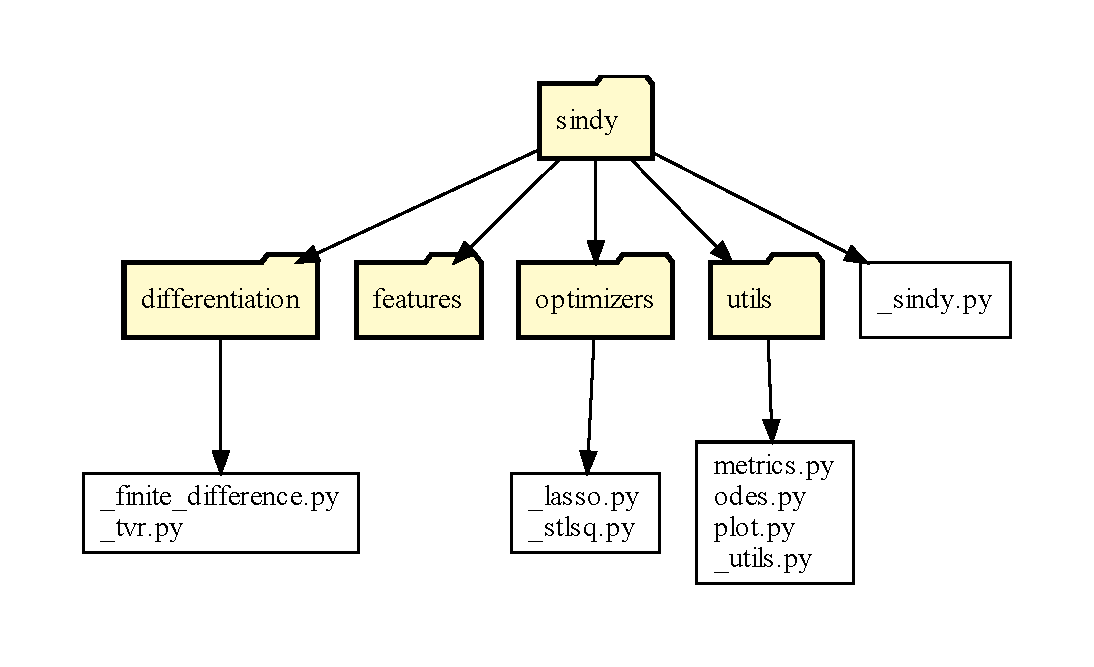
\includegraphics[width=0.85\textwidth]{tree}
\caption{Структура модуля}
\label{fig:tree}
\end{figure}

Для удобства разработки, основные части алгоритма реализованы в отдельных подмодулях.

Подмодуль \texttt{optimizers} содержит реализацию алгоритмов разреженной регрессии. В качестве Lasso используется \texttt{sklearn.linear\_model.Lasso} с зафиксированным параметром \texttt{fit\_intercept=False}, который убирает свободный член из формулы регрессии (считаем, что он задается в матрице признаков, если необходим). STLSQ реализован как \texttt{sklearn.base.RegressorMixin}.

Подмодуль \texttt{differentiation} содержит алгоритмы численного дифференцирования, \texttt{\_finite\_difference.py} --- метод конечных разностей, \texttt{\_tvr.py} --- методы регуляризации полной вариации. Первый метод назван \texttt{FastTVR}, так как не является итеративным и содержит только одну процедуру решения СЛАУ, второй метод --- просто \texttt{TVR}. При описании результатов в подразделе~\ref{section:results} методы указаны именно с этими именами. Все алгоритмы дифференцирования реализованы как \texttt{sklearn.base.TransformerMixin}, методы регуляризации полной вариации используют матрицы дискретных операторов в явном виде.

Подмодуль \texttt{features} не содержит никаких реализаций, поскольку в работе в итоге исследовались только системы с полиномиальными правыми частями, и для получения матрицы признаков использовался \texttt{sklearn.preprocessing.PolynomialFeatures}.

Подмодуль \texttt{utils} содержит различные вспомогательные классы и функции. В частности метрики, используемые системы ОДУ, функции для генерации и визуализации данных.

Алгоритм идентификации реализован в \texttt{\_sindy.py} как \texttt{sklearn.base.BaseEstimator}. \enquote{Обученный} алгоритм может предсказывать значения левых частей системы, а также описать саму систему или составить экземпляр класса \texttt{sindy.utils.Equation}, который затем можно эволюционировать для получения траектории.

Исходный код программной разработки доступен в репозитории по ссылке в приложении А.

    \section{РЕЗУЛЬТАТЫ РАБОТЫ}

\subsection{Результаты}
\label{section:results}

\subsubsection{Анализ методов разреженной регрессии}

Для анализа алгоритмов линейной регрессии при помощи \texttt{sklearn.datasets.make\_regression} сгенерирован датасет из 100 объектов, с одним значением целевой переменной. Каждый объект описывается 100 признаками, из которых значимыми являются только 10. К значениям признаков добавлен гауссовский шум с дисперсией 5. Визуализация истинных значений коэффициентов представлена на рисунке~\ref{fig:regr:coef}.

\begin{figure}
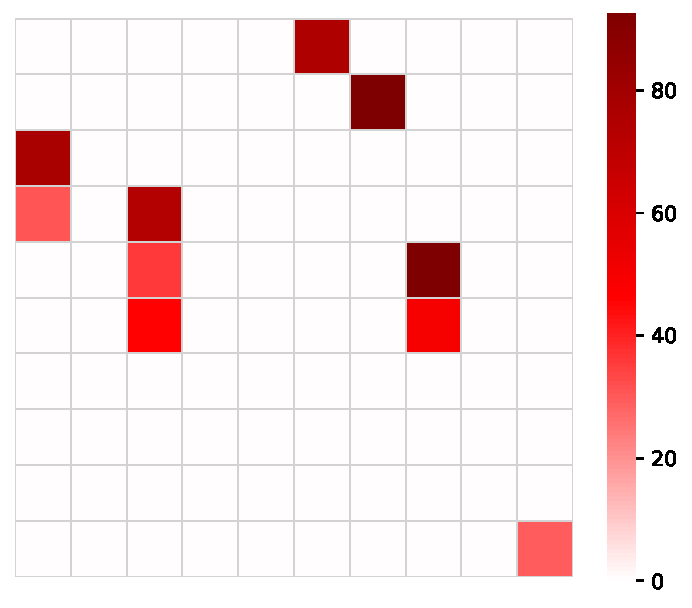
\includegraphics[width=.5\textwidth]{regr/coef}
\caption{Истинные коэффициенты}
\label{fig:regr:coef}
\end{figure}

В качестве контрольного примера, на рисунке~\ref{fig:regr:linear} приведены результаты работы обычной линейной регрессии без регуляризации. Для оценки результатов самой регрессии используются такие метрики, как максимальная ошибка, средняя абсолютная ошибка, среднеквадратичная ошибка, коэффициент детерминации. Как и ожидалось, такой метод хорошо предсказывает значения целевой переменной, но совершенно не справляется с отбором признаков. Хорошие результаты предсказаний также говорят о том, что этот метод подстраивается под шум.

\begin{figure}
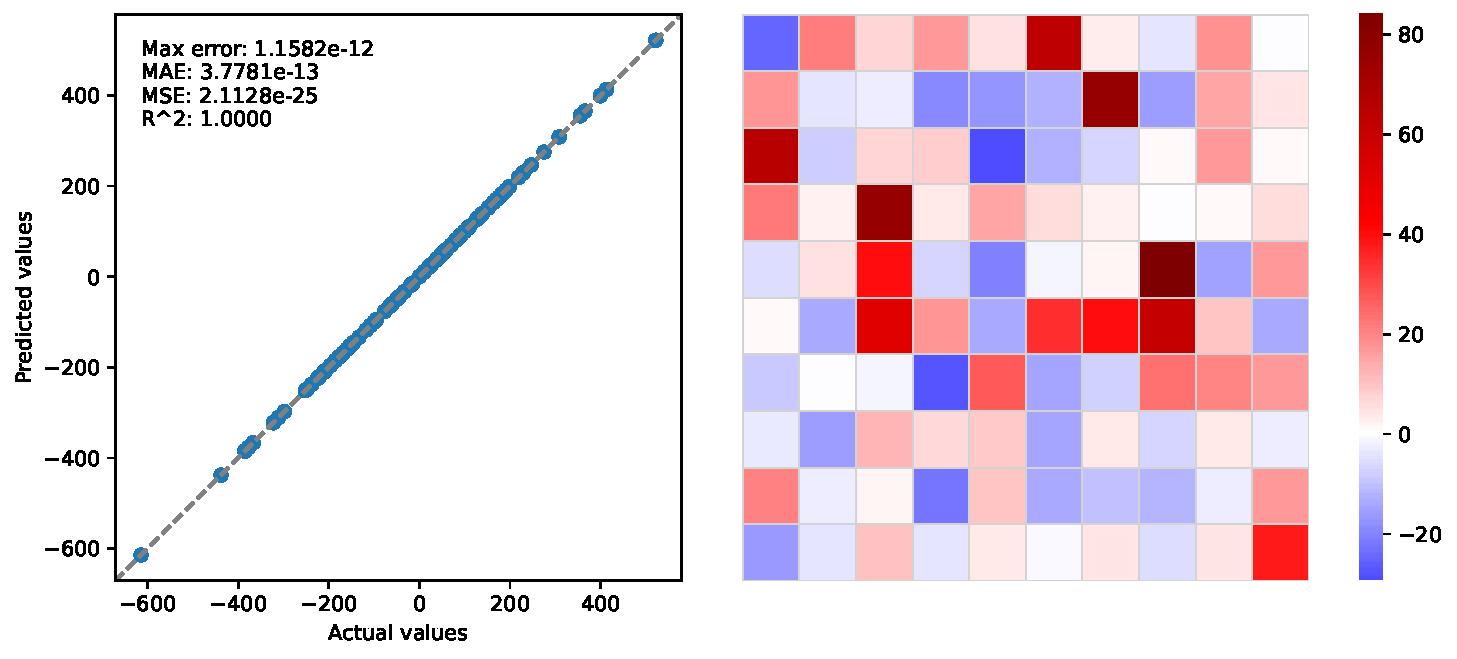
\includegraphics[width=\textwidth]{regr/linear}
\caption{Результаты работы линейной регрессия без регуляризации}
\label{fig:regr:linear}
\end{figure}

На рисунке~\ref{fig:regr:lasso} приведены результаты работы Lasso --- линейной регрессии с $L_1$ регуляризацией. Коэффициент регуляризации $\alpha = 1$.

\begin{figure}
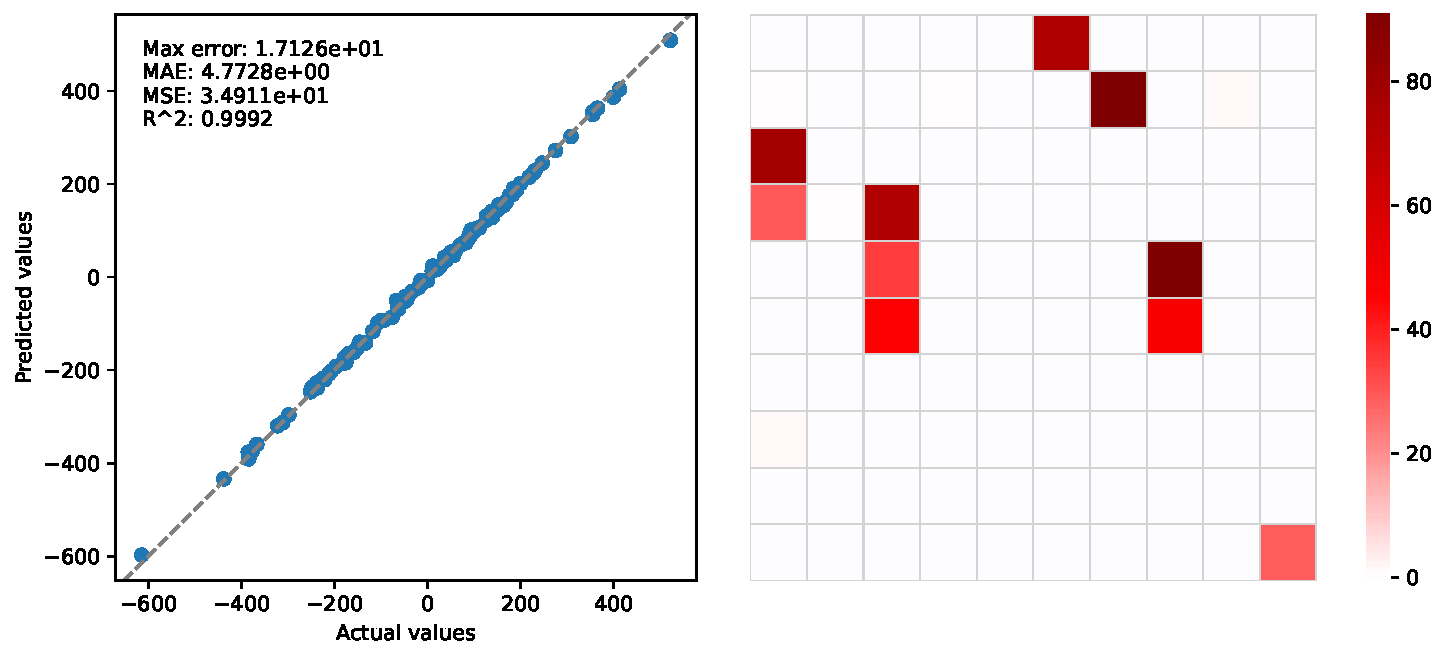
\includegraphics[width=\textwidth]{regr/lasso}
\caption{Результаты работы Lasso}
\label{fig:regr:lasso}
\end{figure}

На рисунке~\ref{fig:regr:stlsq} приведены результаты работы STLSQ. Пороговое значение $\alpha = 2$.

\begin{figure}
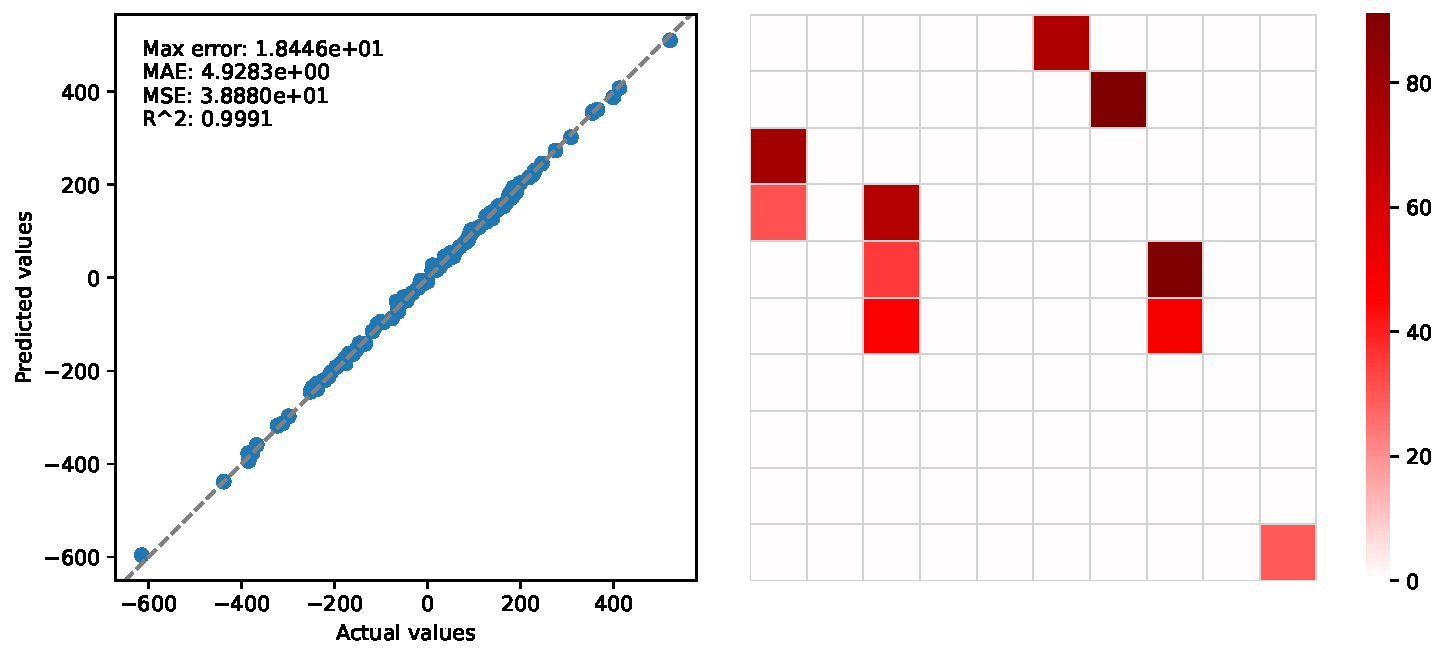
\includegraphics[width=\textwidth]{regr/stlsq}
\caption{Результаты работы STLSQ}
\label{fig:regr:stlsq}
\end{figure}

В результате тестирования можно сказать, что методы разреженной регрессии действительно справляются с поставленной задачей. Ценой этому служит необходимость подбора параметров и уменьшение точности. Но, так как они используются в структурной идентификации, отбор признаков является более важным результатом, чем качество предсказаний.

    \subsubsection{Анализ методов численного дифференцирования}

Использование методов численного дифференцирования, основанных на регуляризации полной вариации, осложняется наличием у этих методов параметров. Оба метода имеют параметр, отвечающий за степень регуляризации, второй метод, будучи итеративным, также содержит ограничение на число итераций. Поэтому в данном пункте будут проанализированы эти методы, проведено сравнение с методом конечных разностей и выявлены закономерности влияния параметров на конечный результат.

Параметр $\alpha$ --- коэффициент регуляризации --- несет одинаковую функцию в обоих методах: определяет насколько сильно будет подвергаться регуляризации процесс дифференцирования. Так как речь идет о регуляризации полной вариации, его влияние на производную очевидно: при увеличении $\alpha$, полная вариация производной будет уменьшаться, приводя к \enquote{уплощению} графика, до тех пор, пока он не выродится в прямую линию. Это подтверждает пример с дифференцированием синусоиды (без добавочного шума) на рисунке~\ref{fig:dif:alpha}.

\begin{figure}
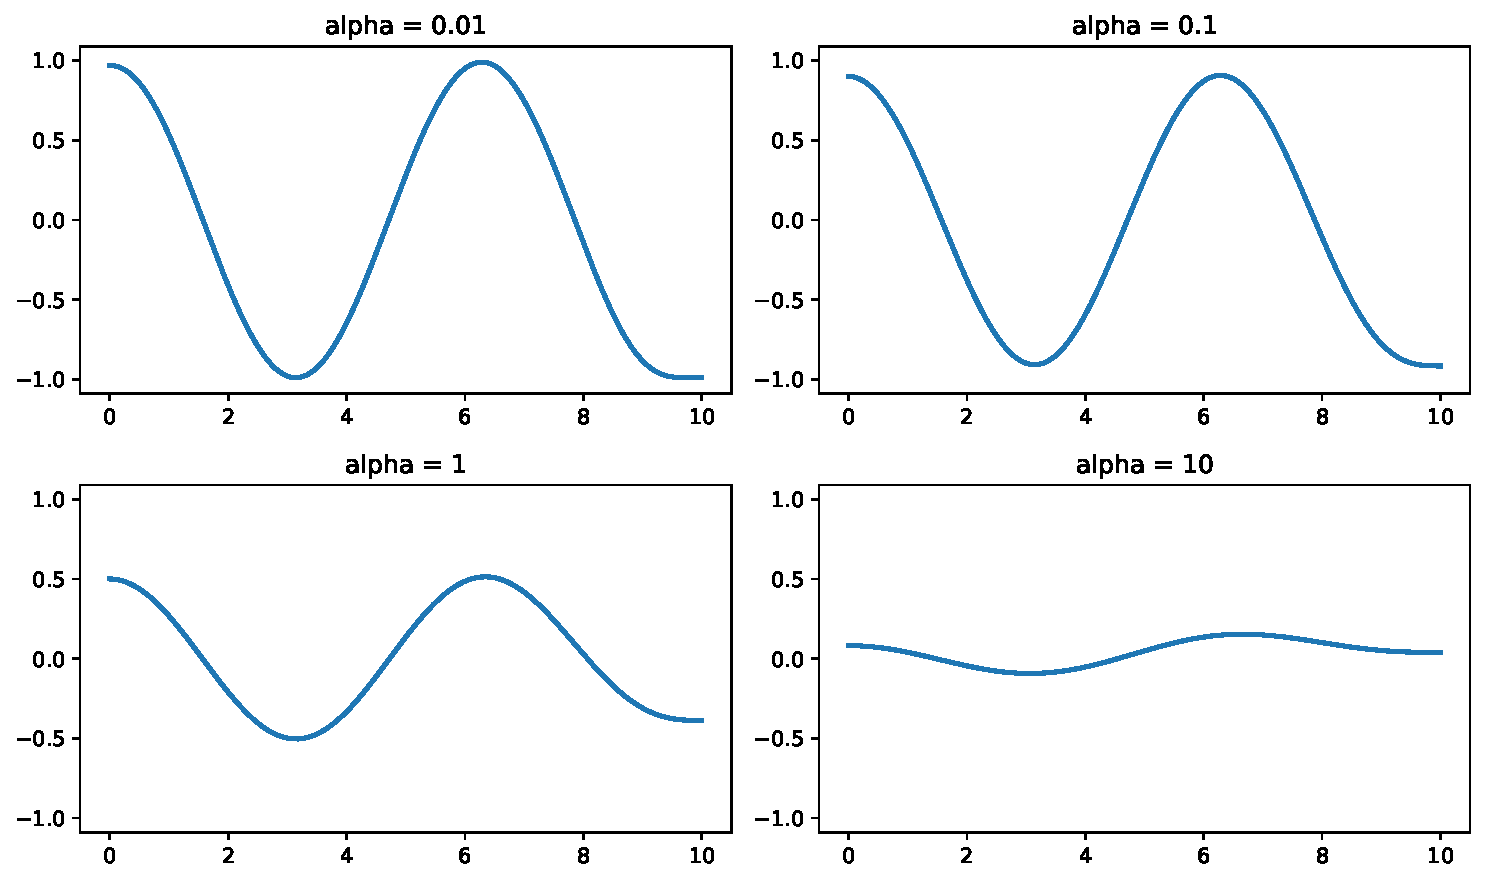
\includegraphics[width=0.9\textwidth]{dif/alpha}
\caption{Результаты дифференцирования при различных значениях параметра $\alpha$}
\label{fig:dif:alpha}
\end{figure}

Для итеративного метода параметром также является число итераций. Итеративный процесс сходится к некоторому стационарному состоянию, пример значений производной той же самой синусоиды (уровень шума --- $0.05$) на разных итерациях показан на рисунке~\ref{fig:dif:max_iter}. Так как в этом случае речь идет о полной вариации полученной производной, на графиках видно увеличение ступенчатости --- количества и размеров областей с постоянными значениями, которые имеют нулевую вариацию.

\begin{figure}
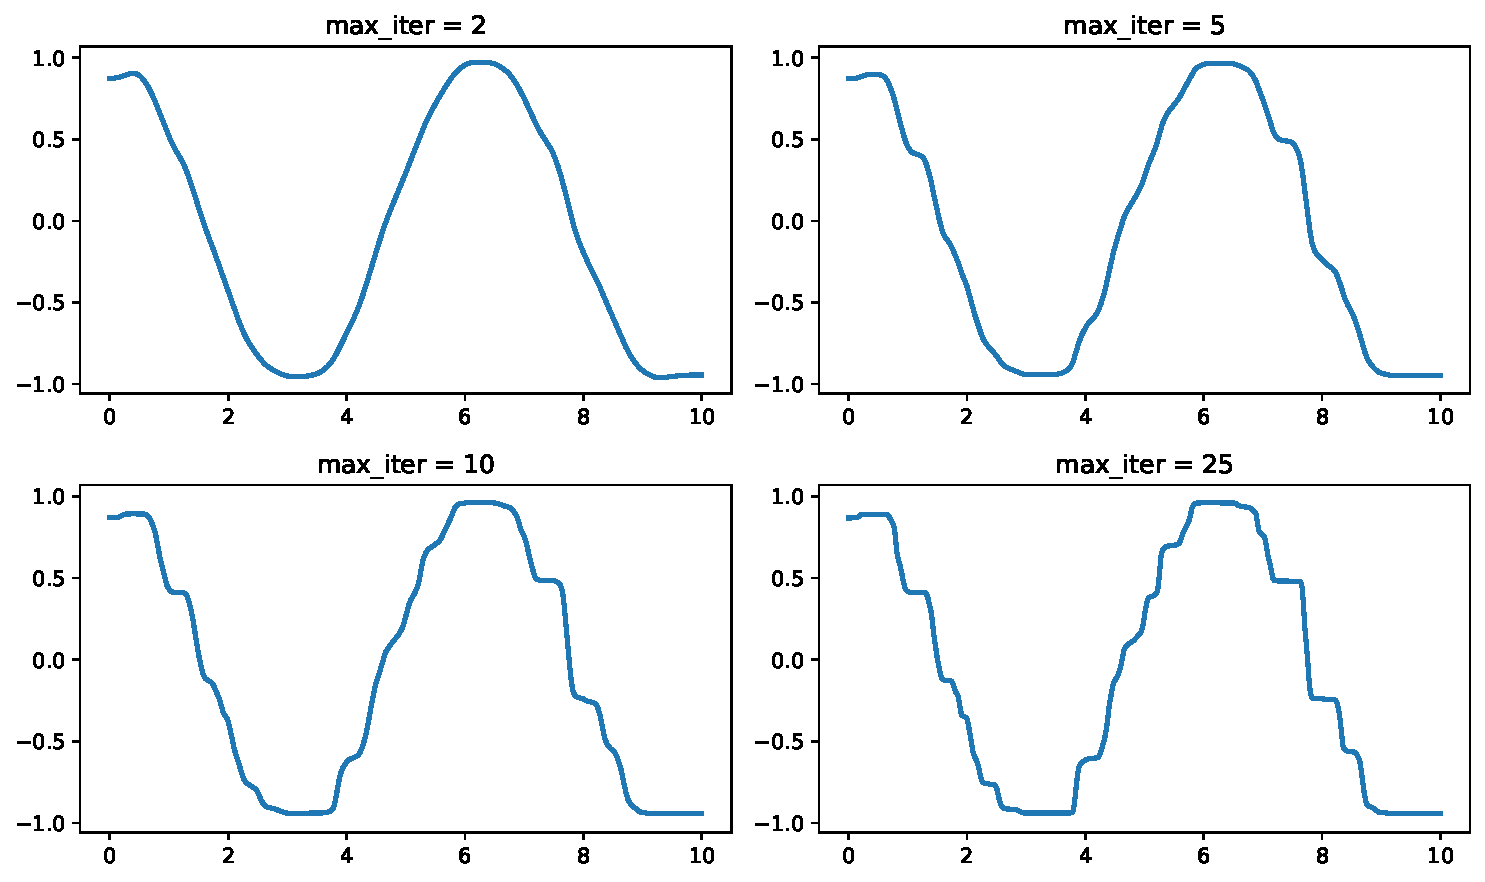
\includegraphics[width=0.9\textwidth]{dif/max_iter}
\caption{Результаты дифференцирования на различных итерациях}
\label{fig:dif:max_iter}
\end{figure}

Рассмотрим подробный анализ обоих методов для трех тестовых функций.

\paragraph{Простая функция с непрерывной производной}

В качестве простой функции с непрерывной производной выбрана функция $sin(x)$ на отрезке $[0, 10]$. Она представлена на рисунке~\ref{fig:dif:sin}.

\begin{figure}
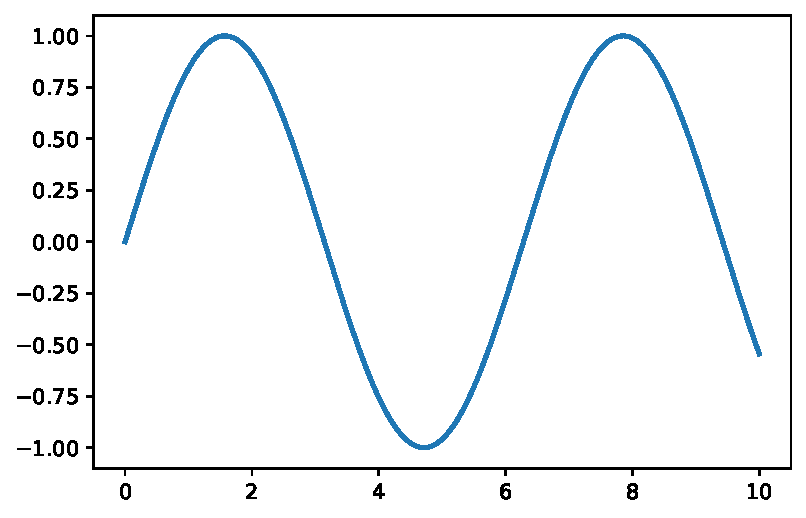
\includegraphics[width=0.5\textwidth]{dif/sin}
\caption{Функция $sin(x)$}
\label{fig:dif:sin}
\end{figure}

Для каждого метода рассмотрим среднюю абсолютную ошибку между результатом дифференцирования и точной производной для:
\begin{itemize}
\item различных разбиений отрезка и фиксированных параметрах,
\item различных уровней шума и фиксированных параметрах,
\item различных величин одного из параметров,
\item комбинаций уровней шума и значений параметра.
\end{itemize}

На рисунке~\ref{fig:dif:sin_fast_tvr} представлено тестирование первого метода.

\begin{figure}
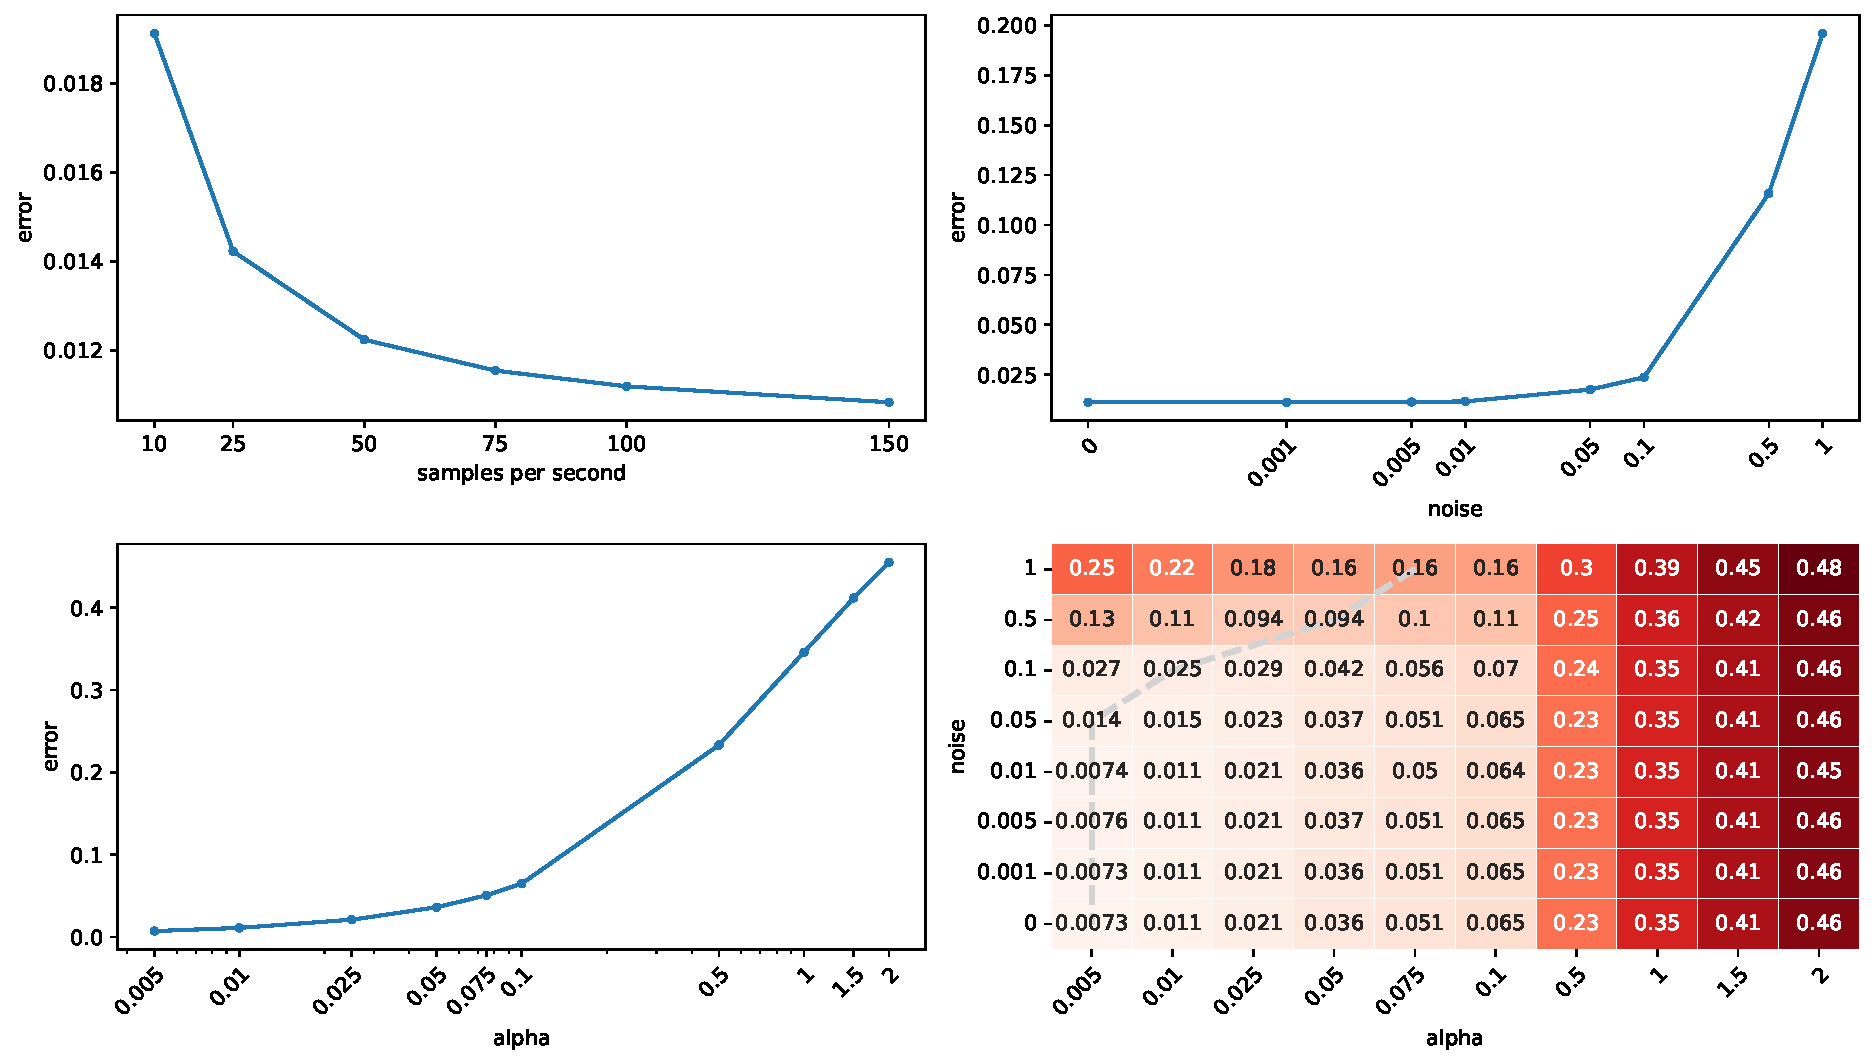
\includegraphics[width=\textwidth]{dif/sin_fast_tvr}
\caption{Тестирование первого метода дифференцирования}
\label{fig:dif:sin_fast_tvr}
\end{figure}

Увеличение разбиения ожидаемо приводит к увеличению точности. Увеличение уровня шума при неизменных параметрах --- к ухудшению результата, возникает задача подбора параметров. Самый большой интерес представляют результаты комбинаций уровня шума и коэффициента регуляризации (серой пунктирной линией обозначена траектория с минимальной ошибкой): большие значения приводят к плохим результатам из-за сильного сглаживания производной, в остальном, можно сказать, что коэффициент регуляризации должен иметь схожий порядок с уровнем шума.

Тестирование второго метода, показанного на рисунке~\ref{fig:dif:sin_tvr}, приводит к схожим результатам. Отдельно стоит отметить влияние на результат числа итераций. При низком уровне шума оно практически не влияет, при больших --- ухудшает результат. Оптимальное число итераций --- 2.

\begin{figure}
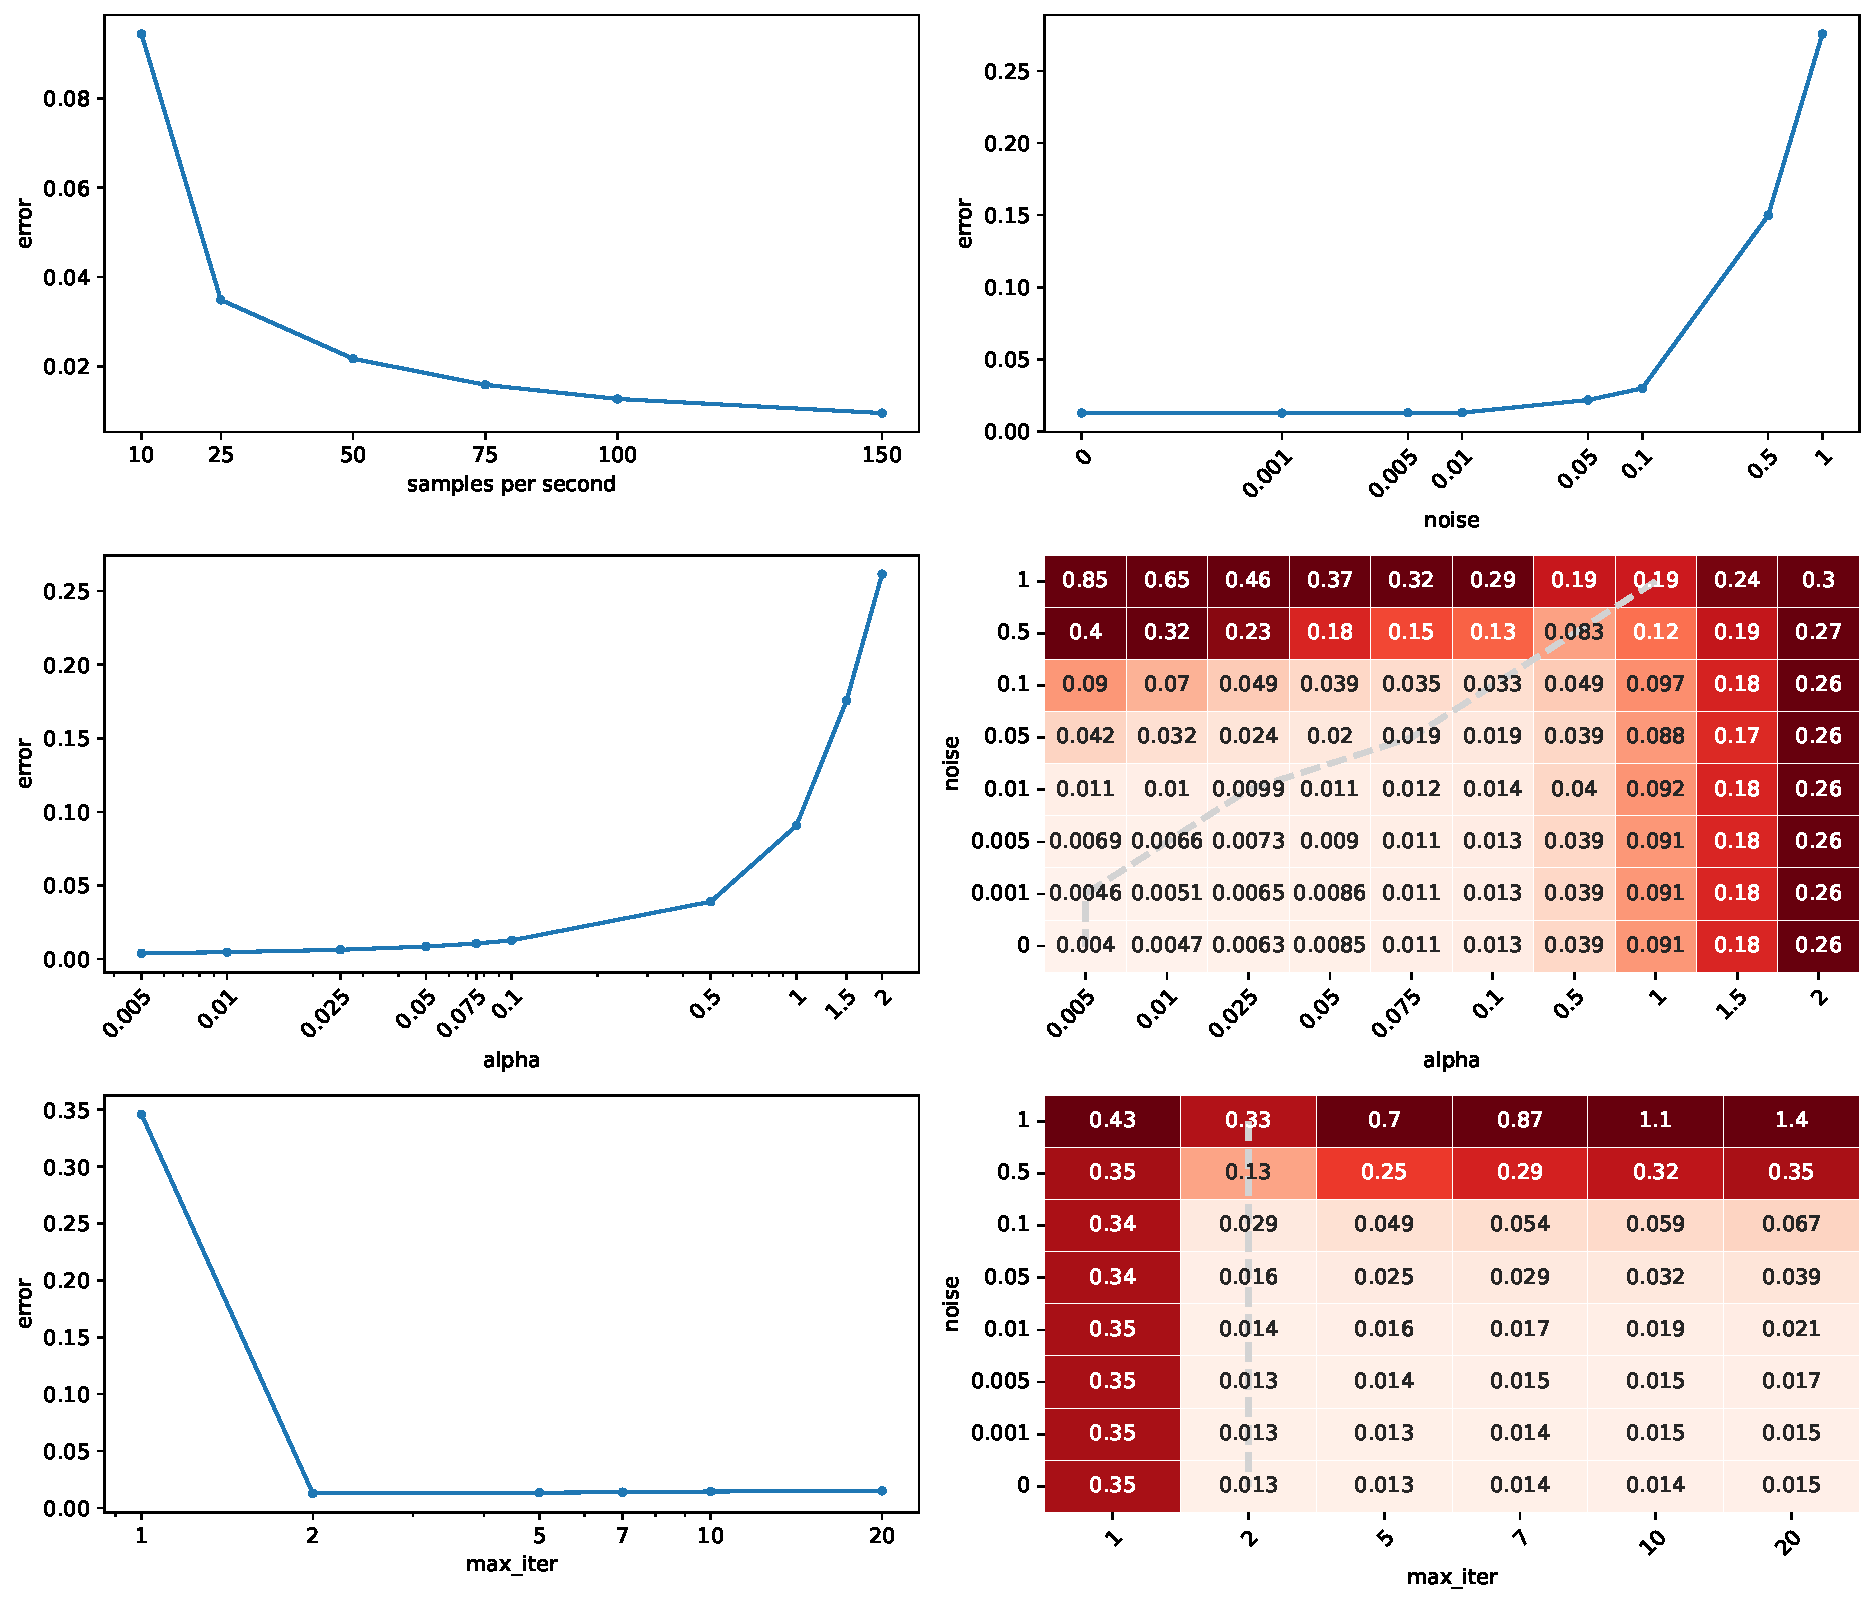
\includegraphics[width=\textwidth]{dif/sin_tvr}
\caption{Тестирование второго метода дифференцирования}
\label{fig:dif:sin_tvr}
\end{figure}

Таким образом можно подобрать параметры для приемлемого дифференцирования данных с различным уровнем шума. Это показано на рисунке~\ref{fig:dif:sin_test}. Столбцы соответствуют различным уровням шума (первый столбец --- точные значения функции и производной), строки --- зашумленным данным, методу конечных разностей, первого и второму методам регуляризации полной вариации соответственно. Очень хорошо видно поведение метода конечных разностей, который перестает справляться с задачей при малейшем шуме.

\begin{figure}
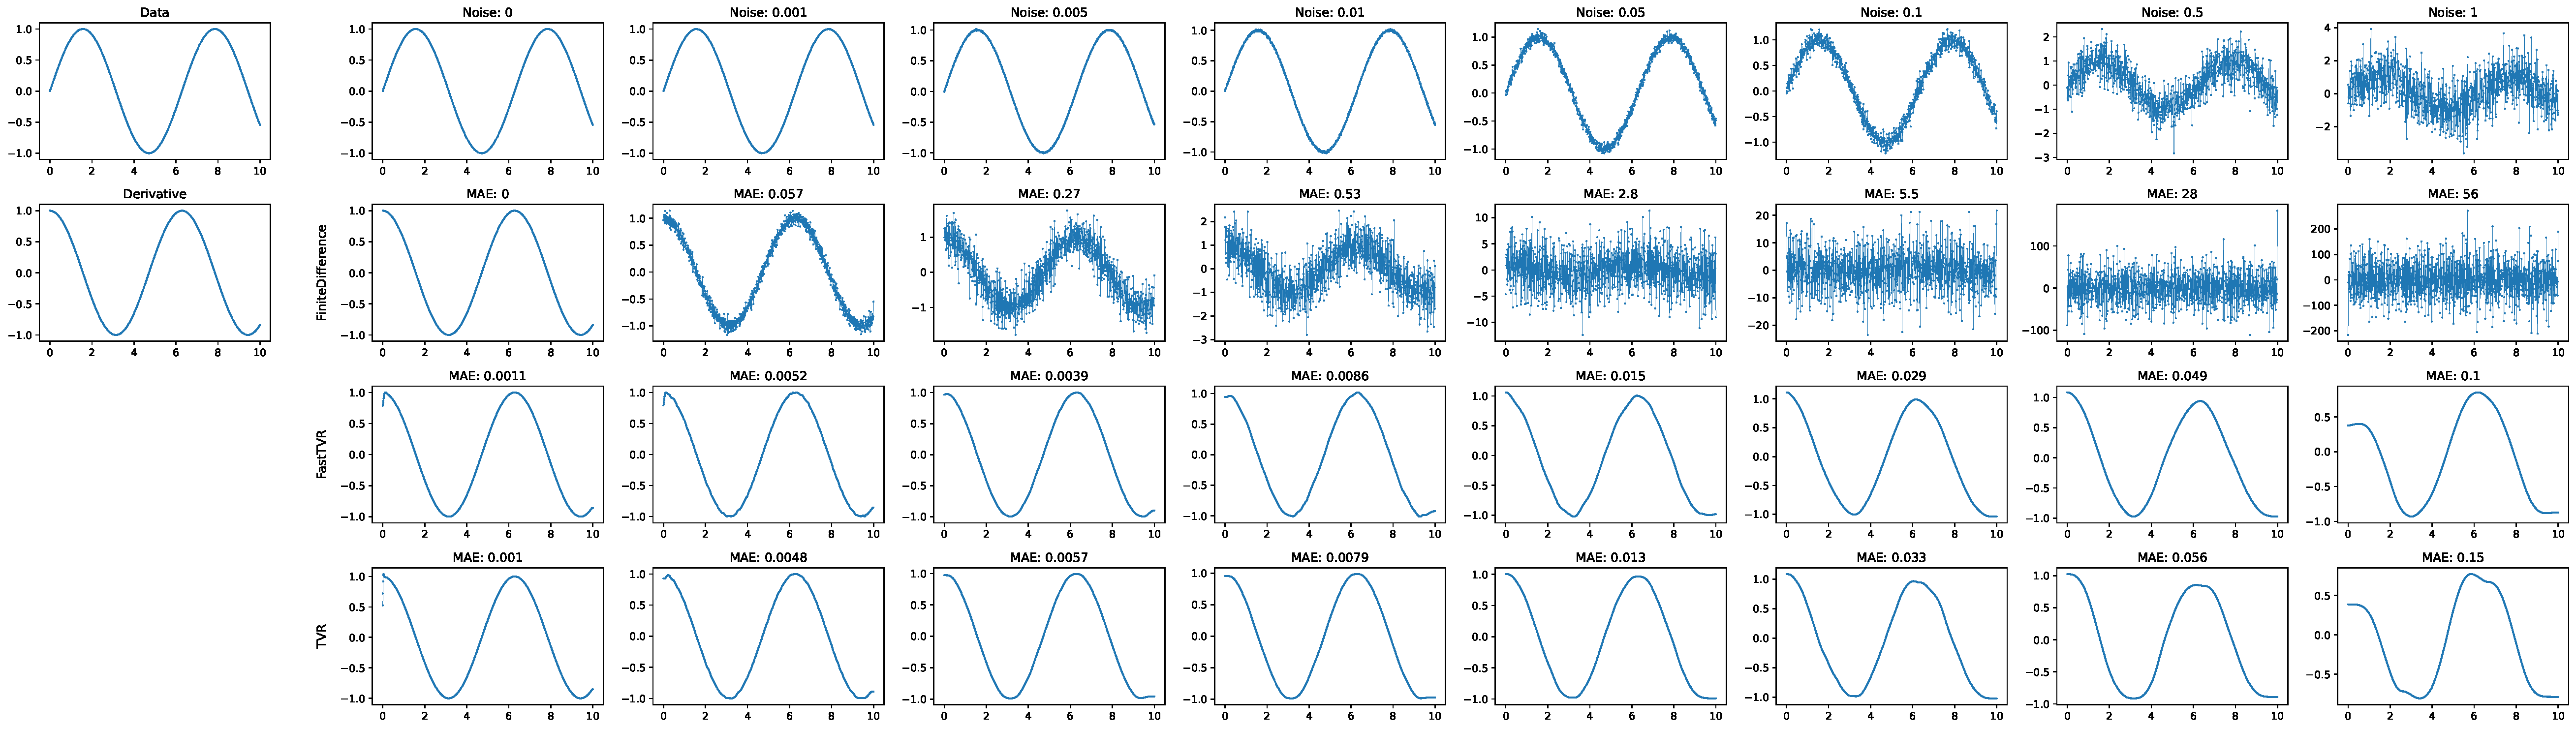
\includegraphics[width=\textwidth]{dif/sin_test}
\caption{Дифференцирование данных с различным уровнем шума}
\label{fig:dif:sin_test}
\end{figure}

\paragraph{Простая функция с разрывной производной}

В качестве функции с разрывной производной выбрана функция модуля $|x|$ на отрезке $[-1, 1]$. Она изображена на рисунке~\ref{fig:dif:abs}.

\begin{figure}
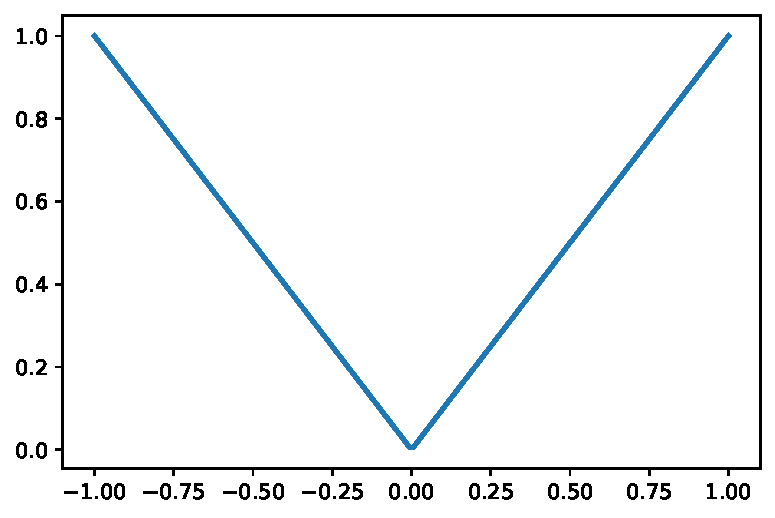
\includegraphics[width=0.5\textwidth]{dif/abs}
\caption{Функция $|x|$}
\label{fig:dif:abs}
\end{figure}

На рисунках~\ref{fig:dif:abs_fast_tvr},~\ref{fig:dif:abs_tvr} представлены результаты тестирования методов. В целом наблюдается довольно похожая картина, однако, более сложный характер функции несколько осложняет дифференцирование. Соотношение между уровнем шума и коэффициентом регуляризации тоже несколько поменялось, теперь коэффициент должен быть на один-два порядка меньше.

\begin{figure}
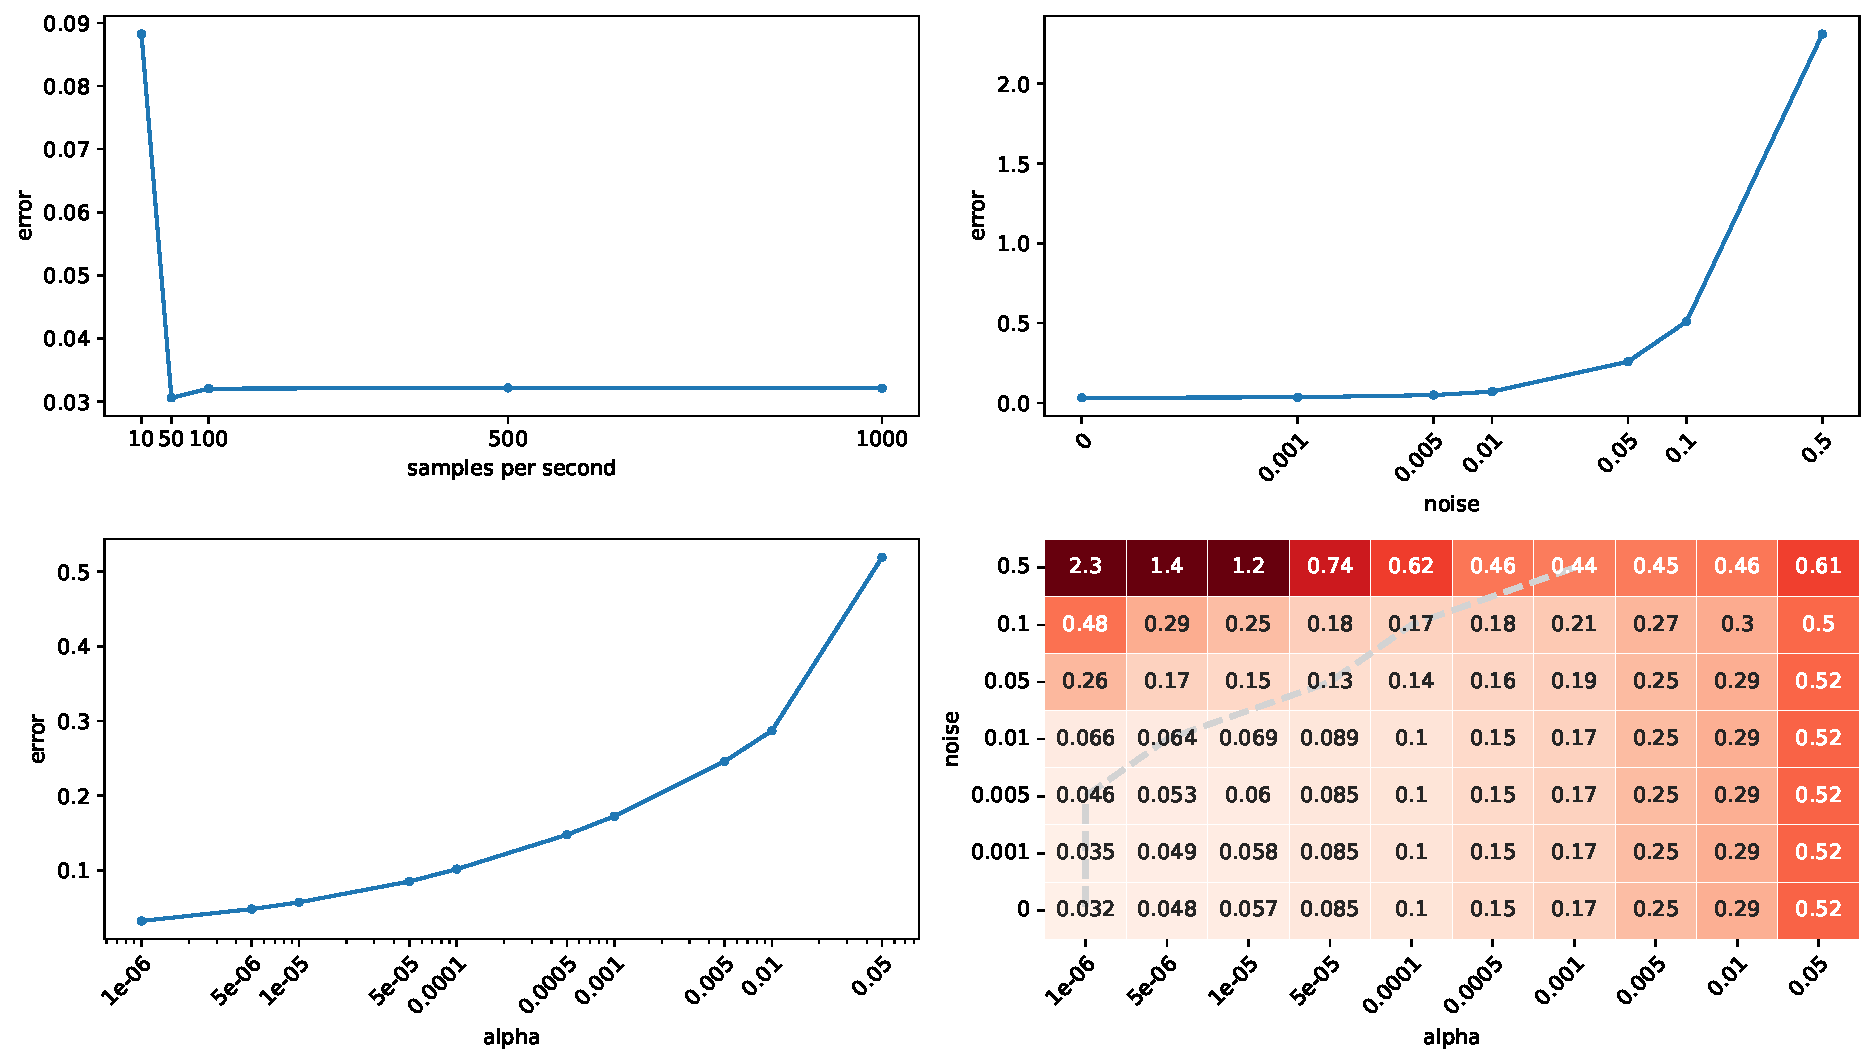
\includegraphics[width=0.9\textwidth]{dif/abs_fast_tvr}
\caption{Тестирование первого метода дифференцирования}
\label{fig:dif:abs_fast_tvr}
\end{figure}

\begin{figure}
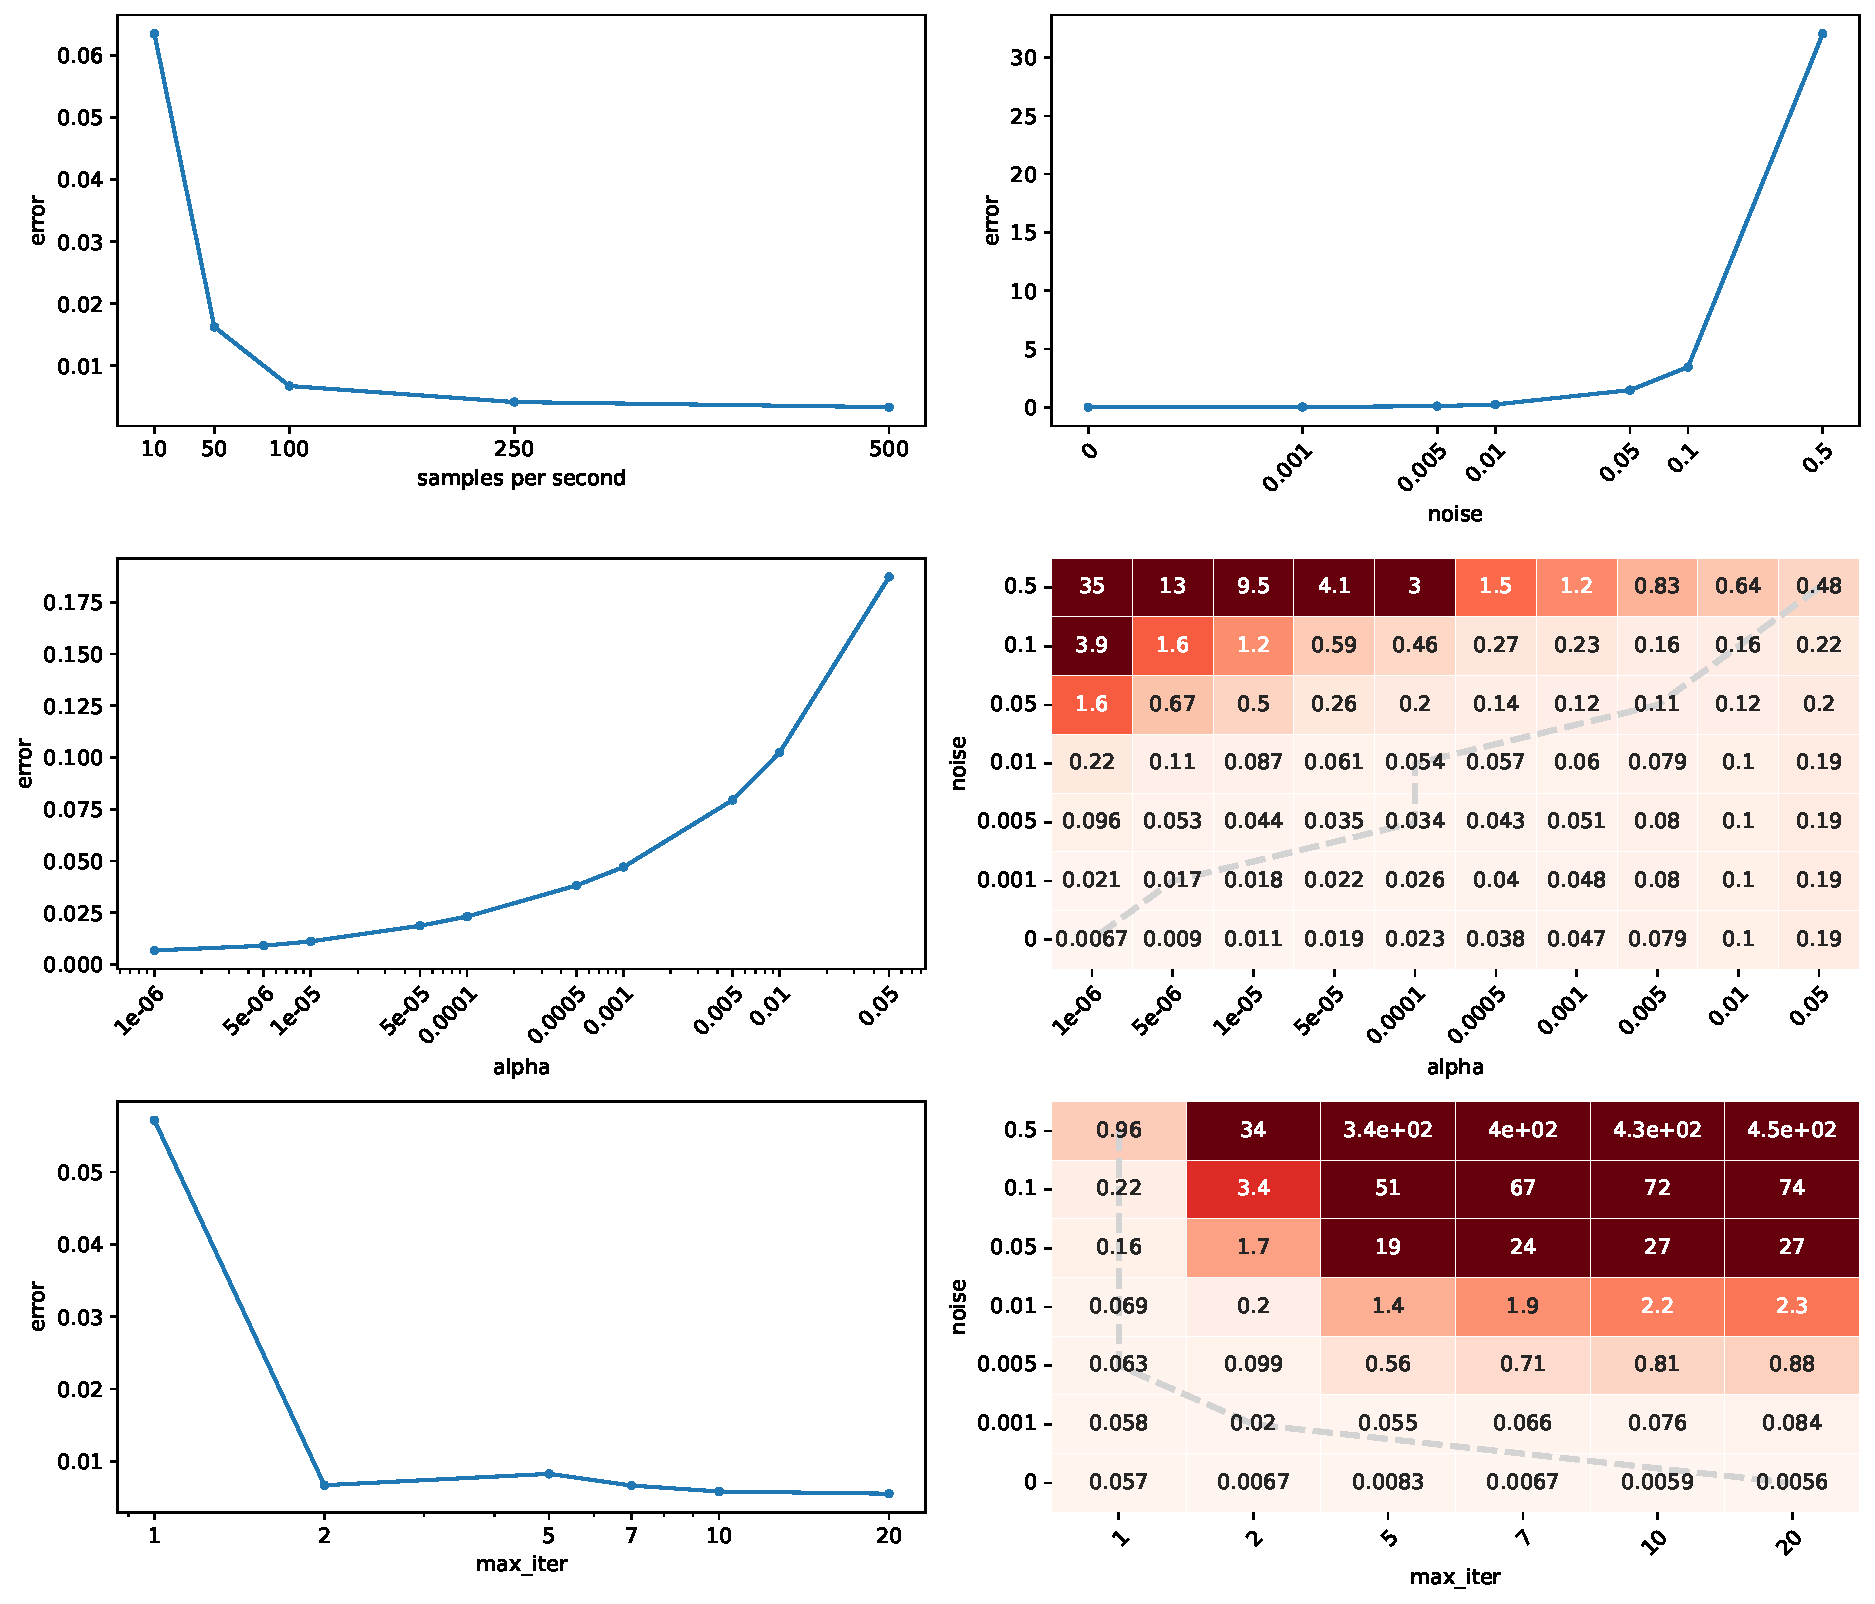
\includegraphics[width=0.9\textwidth]{dif/abs_tvr}
\caption{Тестирование второго метода дифференцирования}
\label{fig:dif:abs_tvr}
\end{figure}

На рисунке~\ref{fig:dif:abs_test} показаны результаты дифференцирования функции с различным уровнем шума. Заметно сглаживание места разрыва с усилением шума, однако, даже когда исходная функция слабо различима, основной характер производной все еще хорошо заметен.

\begin{figure}
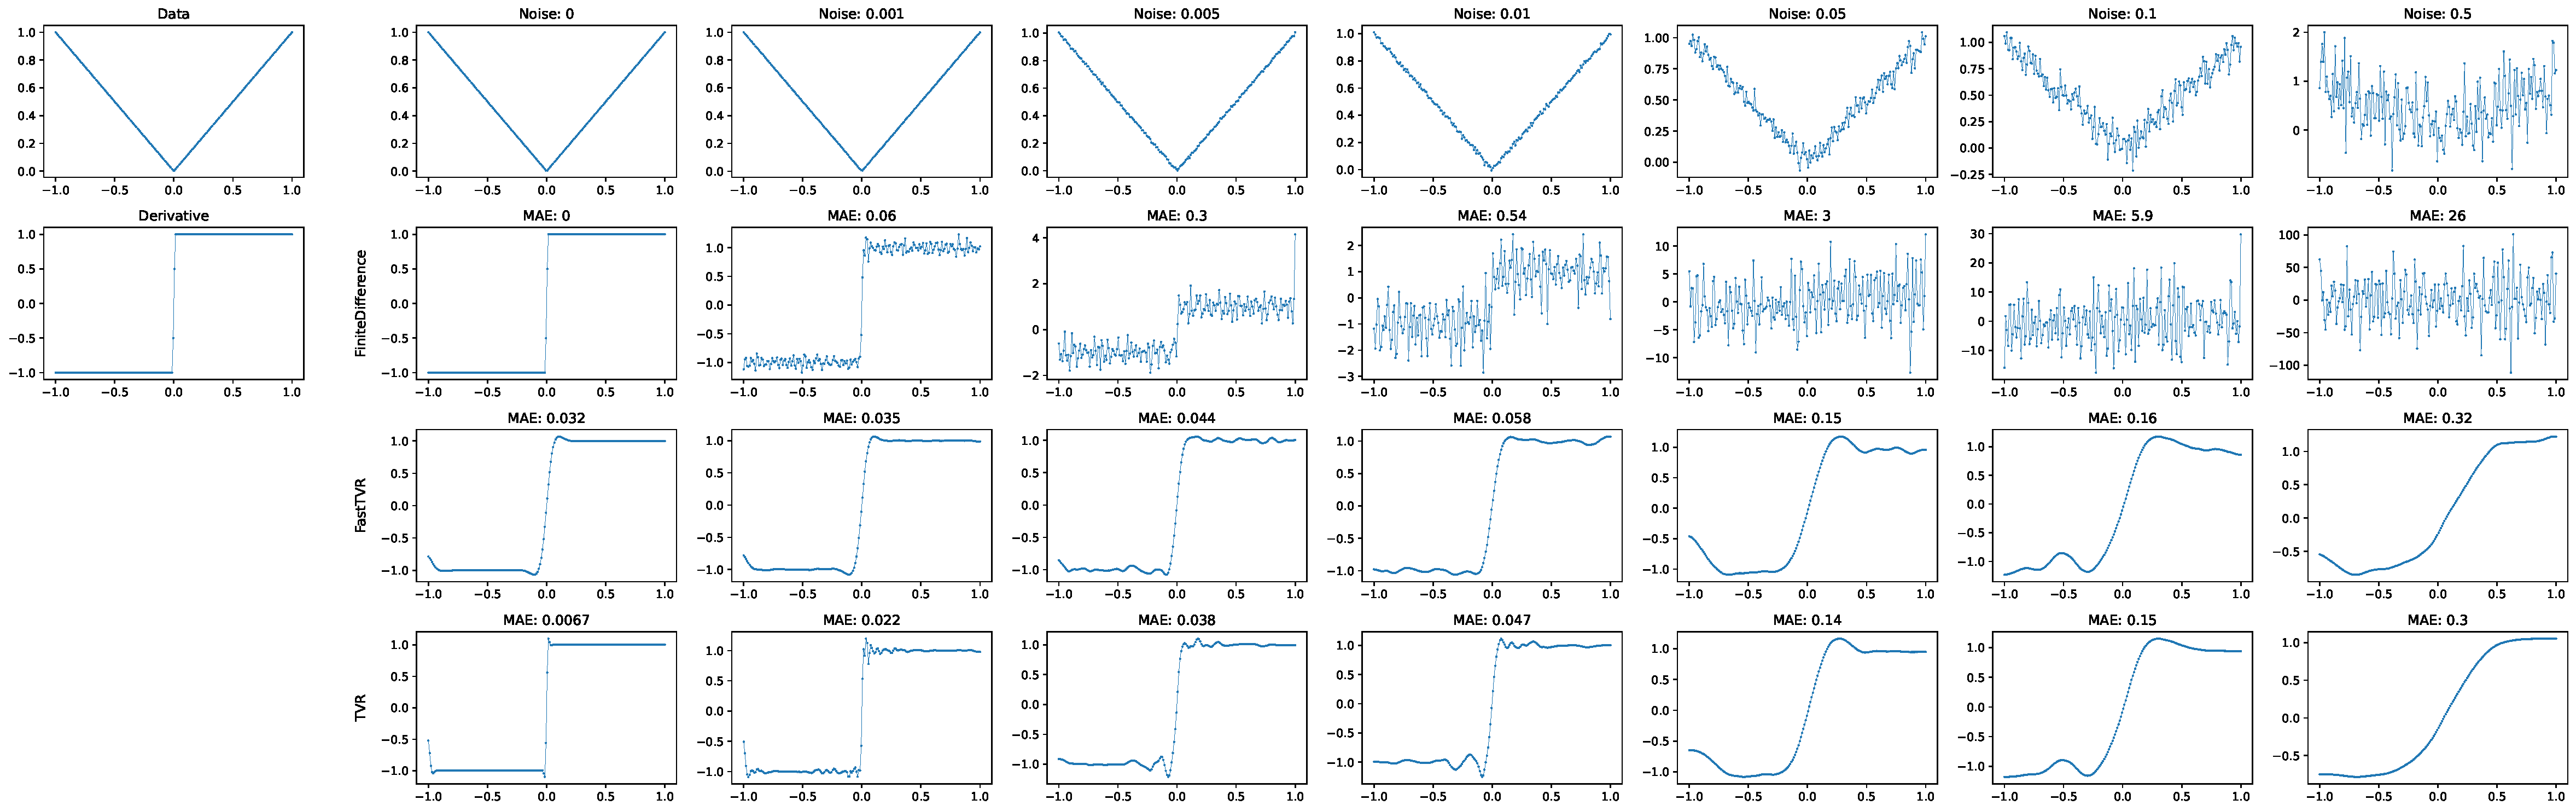
\includegraphics[width=\textwidth]{dif/abs_test}
\caption{Дифференцирование данных с различным уровнем шума}
\label{fig:dif:abs_test}
\end{figure}

\paragraph{Сложная функция с непрерывной производной}

В качестве более сложной функции чем синус, но все еще с непрерывной производной, выбран аттрактор Лоренца --- решение системы Лоренца. Аттрактор изображен на рисунке~\ref{fig:dif:lorenz}.

\begin{figure}
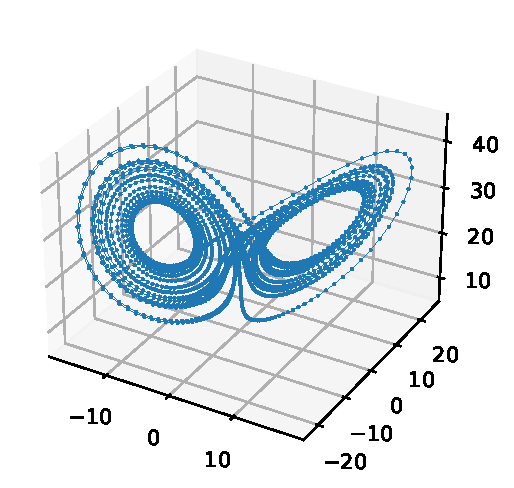
\includegraphics[width=0.5\textwidth]{dif/lorenz}
\caption{Аттрактор Лоренца}
\label{fig:dif:lorenz}
\end{figure}

На рисунках~\ref{fig:dif:lorenz_fast_tvr},~\ref{fig:dif:lorenz_tvr} представлены результаты тестирования методов. Оптимальная величина параметра $\alpha$ упала еще на несколько порядков.

\begin{figure}
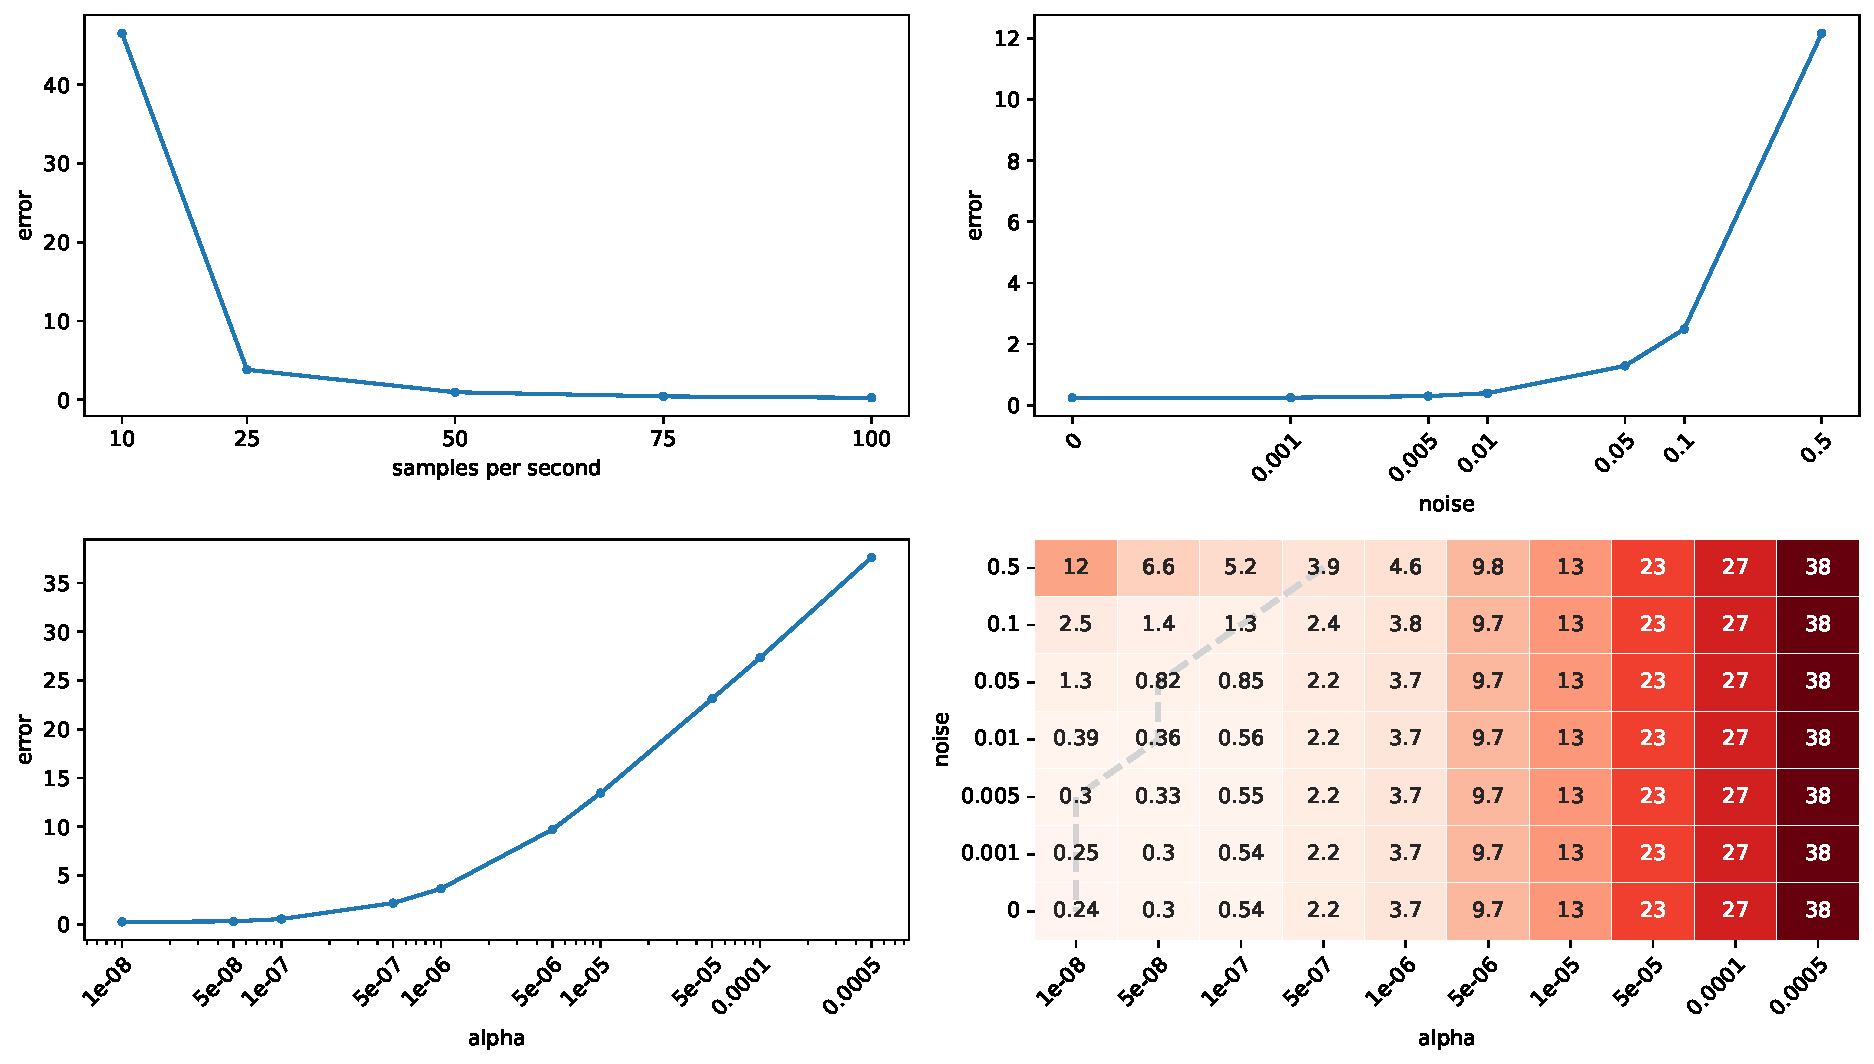
\includegraphics[width=0.9\textwidth]{dif/lorenz_fast_tvr}
\caption{Тестирование первого метода дифференцирования}
\label{fig:dif:lorenz_fast_tvr}
\end{figure}

\begin{figure}
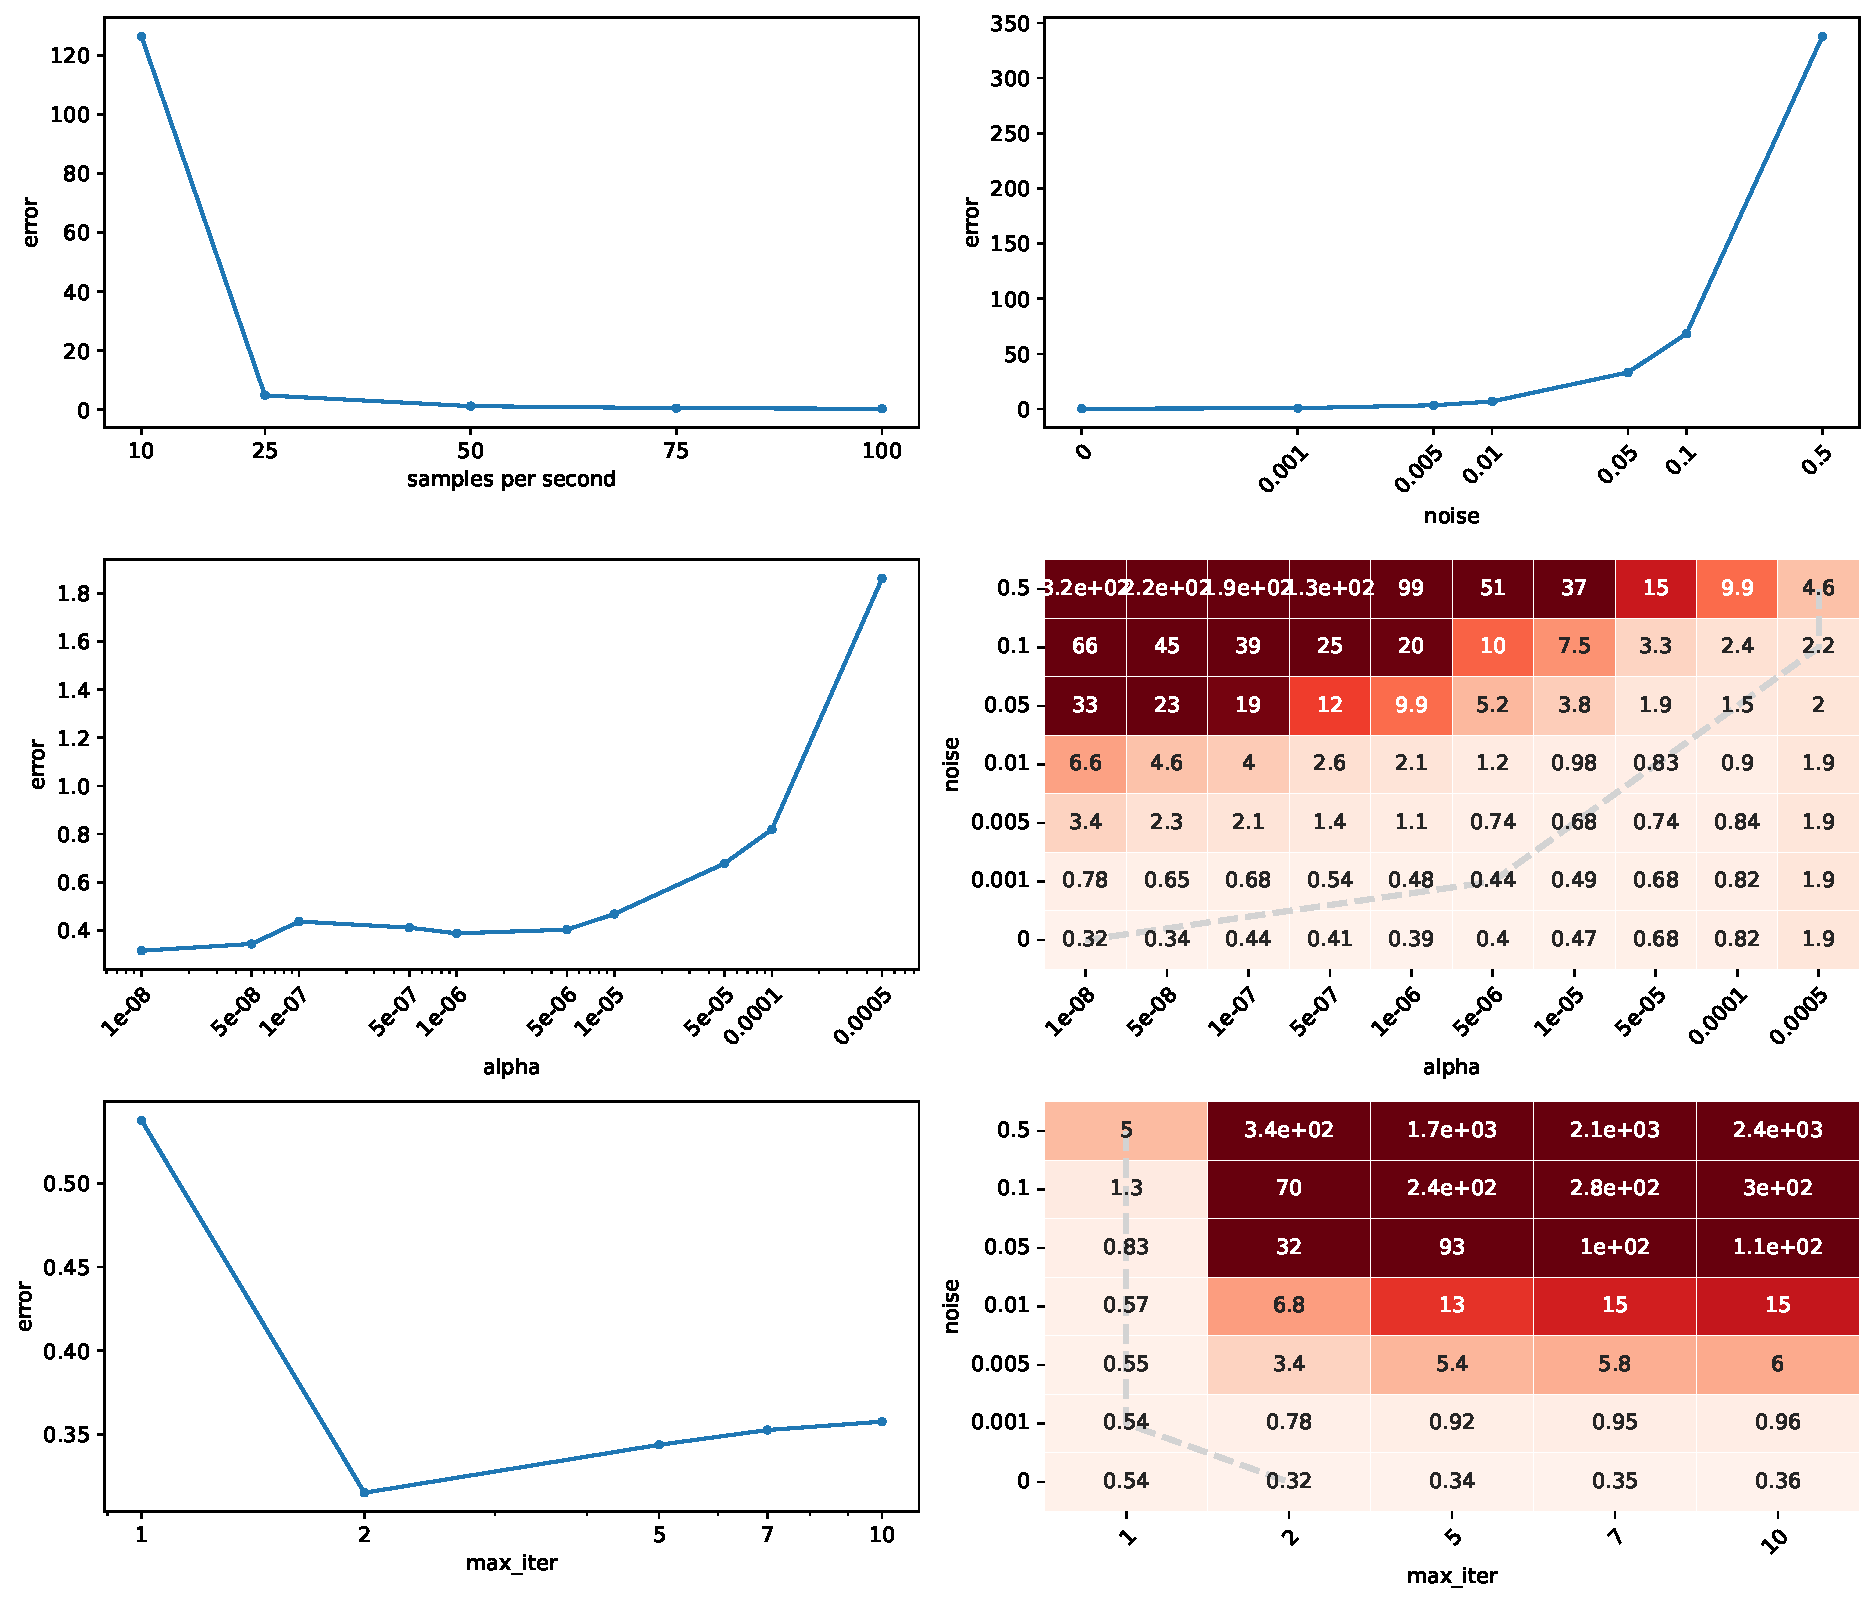
\includegraphics[width=0.9\textwidth]{dif/lorenz_tvr}
\caption{Тестирование второго метода дифференцирования}
\label{fig:dif:lorenz_tvr}
\end{figure}

Однако, как показано на рисунке~\ref{fig:dif:lorenz_test}, функция все еще неплохо дифференцируется, что вызывает уверенность в дальнейшей ее успешной идентификации.

\begin{figure}
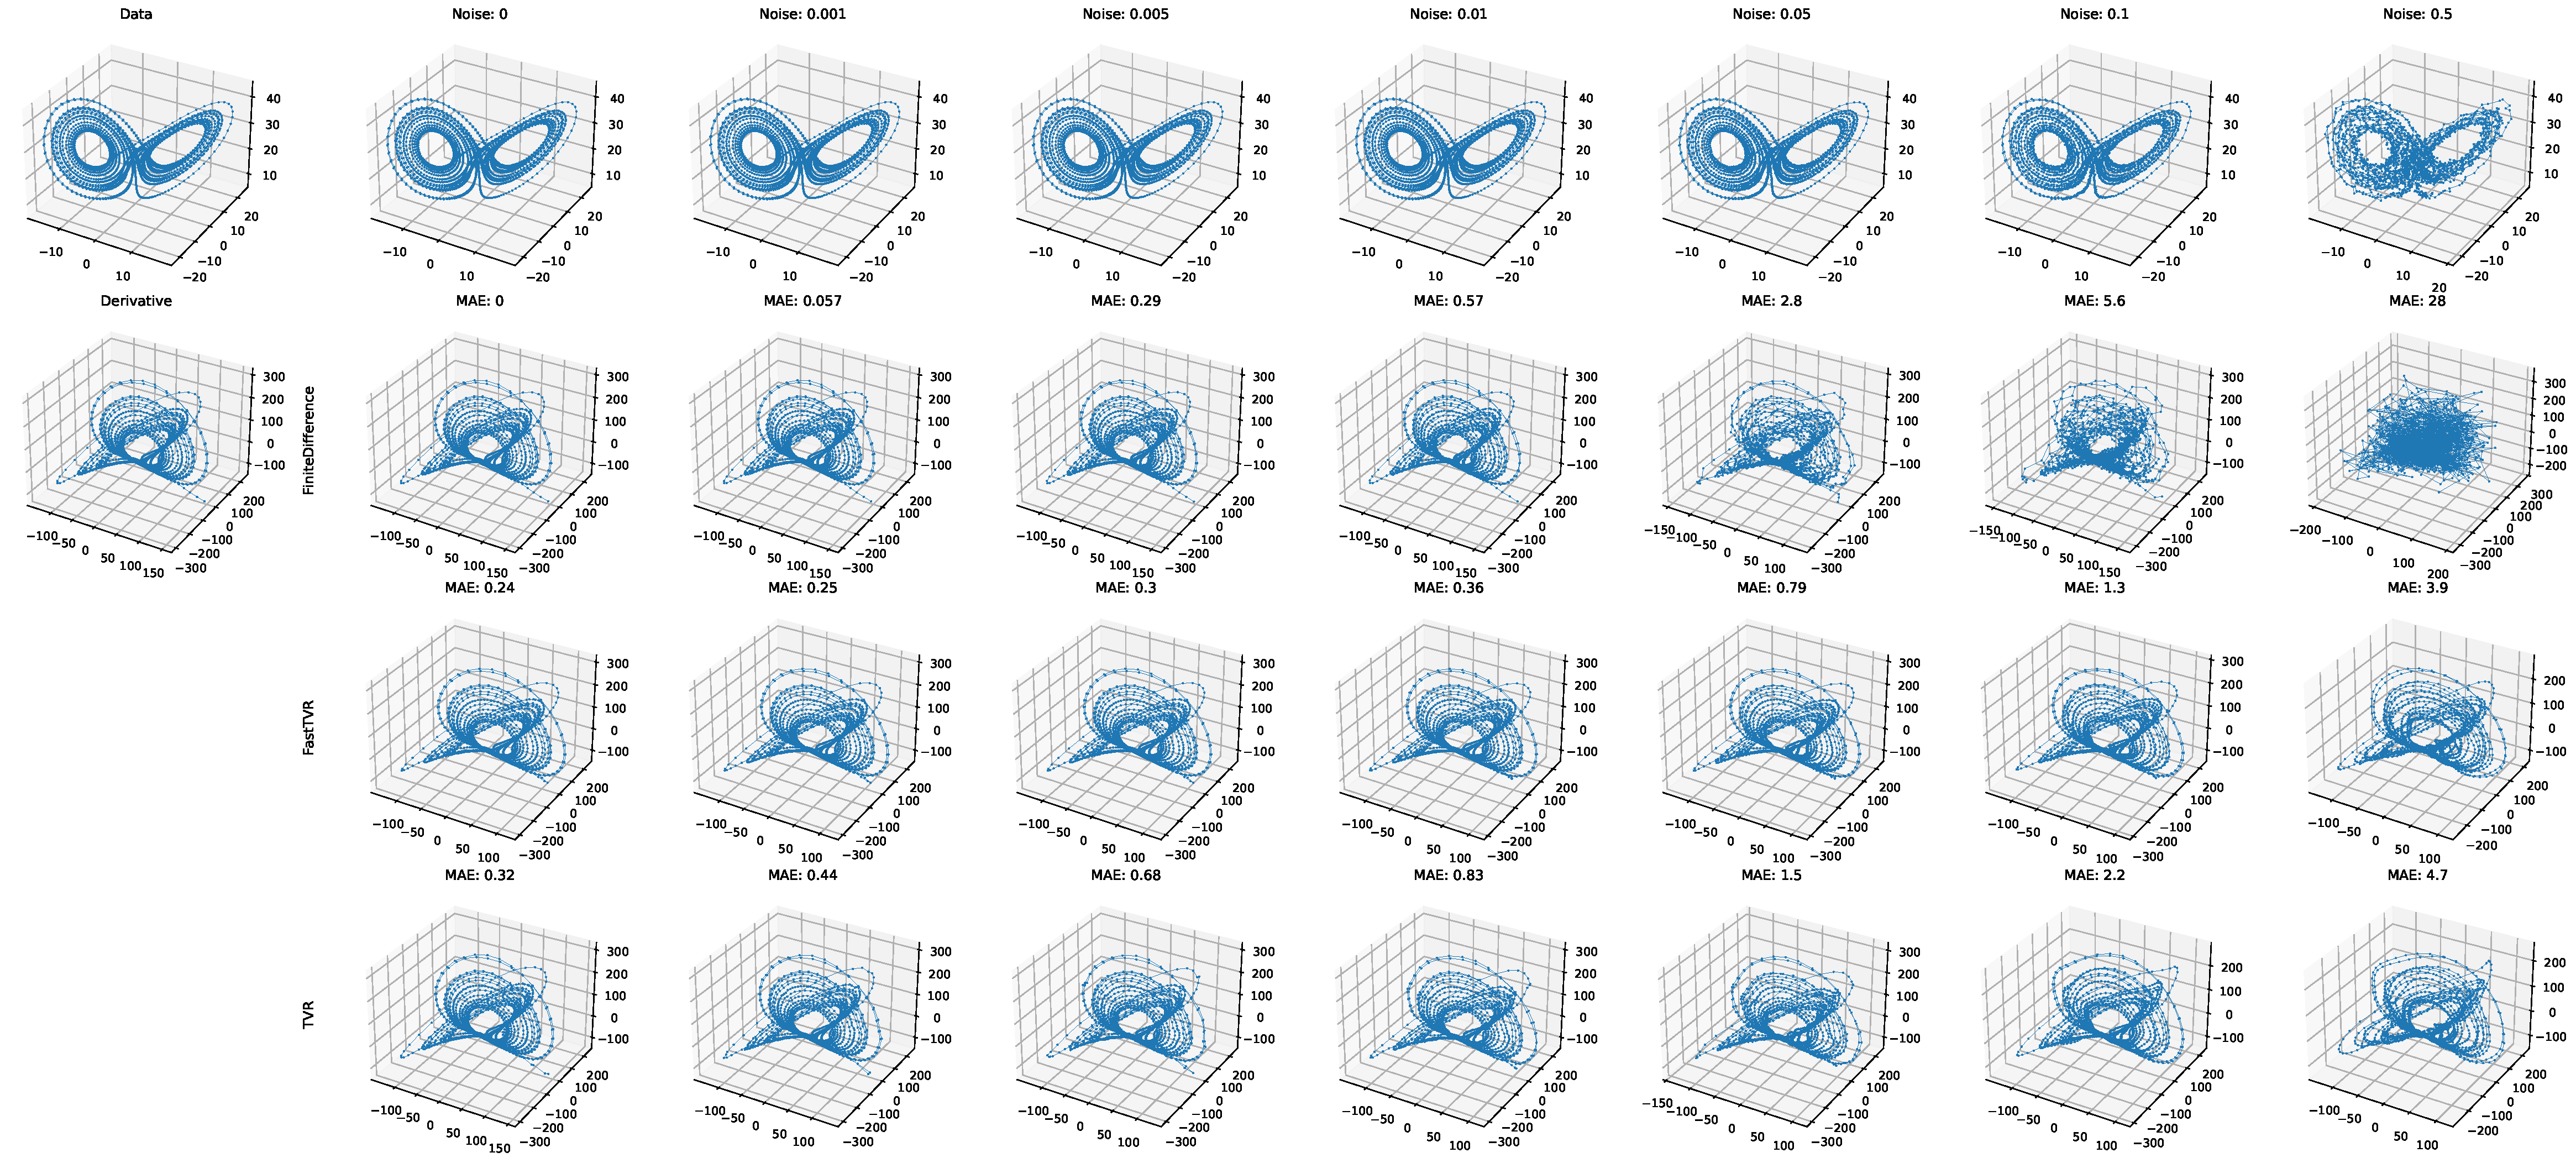
\includegraphics[width=\textwidth]{dif/lorenz_test}
\caption{Дифференцирование данных с различным уровнем шума}
\label{fig:dif:lorenz_test}
\end{figure}

\paragraph{Общие выводы}

По результатам тестирования можно сказать, что успешно дифференцировать зашумленные данные вполне реально. Анализ результатов позволяет сделать некоторое выводы о подборе параметров.

Во-первых, чем больше измерений значений функции в единицу времени дано, тем точнее будет полученная производная. Изменение шага сетки является способом контроля погрешности еще в методе конечных разностей и здесь не теряет свою актуальность. Во-вторых, для итеративного метода дифференцирования оптимальным числом итераций является 2. После первой итерации производная еще не достаточно приняла свою форму, а после третьей и далее она становится слишком ступенчатой. Наконец, более подробно остановимся на коэффициенте регуляризации --- параметре, имеющемся у обоих методов.

Из графиков видно, что порядок коэффициента приблизительно линейно связан с порядком уровня шума. Это подтверждает и рисунок~\ref{fig:dif:alpha_test}, на котором изображены оптимальные траектории параметра $\alpha$ в зависимости от уровня шума для нескольких тестируемых функций (в основном систем ОДУ, которые будут использованы в следующем пункте), серой пунктирной линией изображен примерный тренд.

\begin{figure}
\begin{subfigure}[t]{0.9\linewidth}
	\centering
	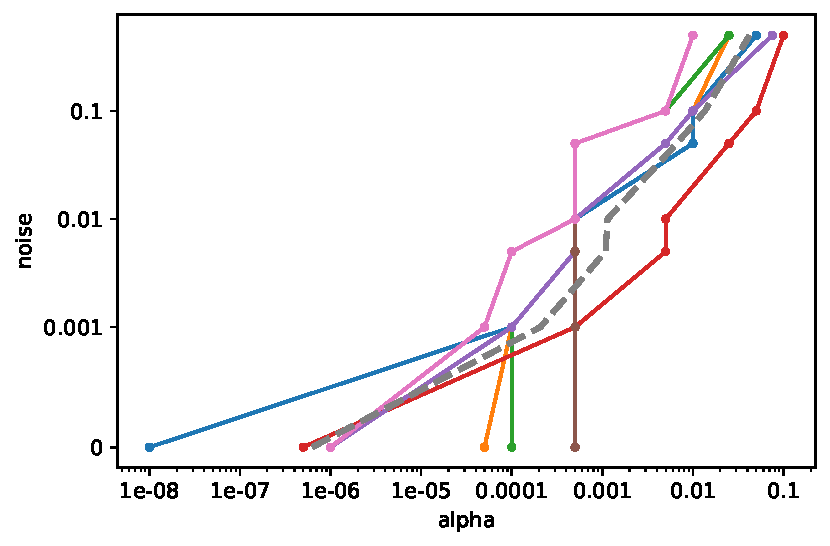
\includegraphics[width=\linewidth]{dif/alpha_fast_tvr}
	\caption{}
\end{subfigure}

\begin{subfigure}[t]{0.9\linewidth}
	\centering
	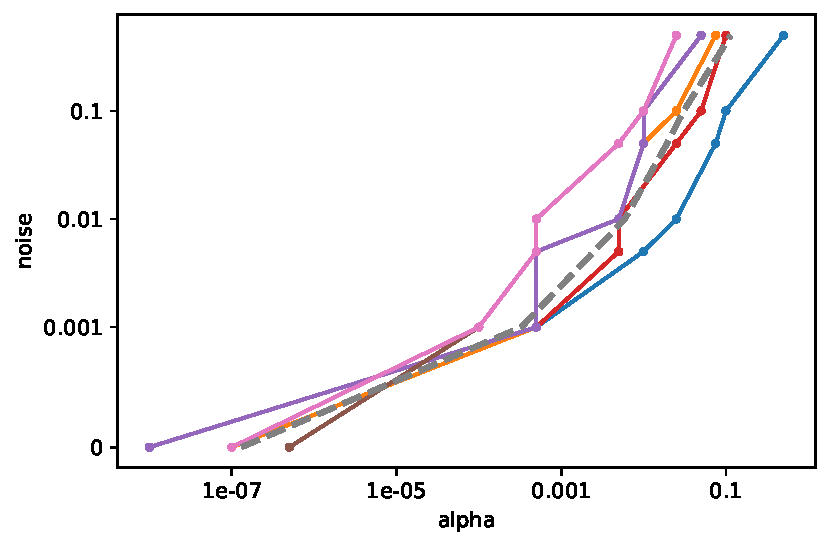
\includegraphics[width=\linewidth]{dif/alpha_tvr}
	\caption{}
\end{subfigure}
\caption{Оптимальные значения параметра $\alpha$: a) для первого метода; б) для второго метода}
\label{fig:dif:alpha_test}
\end{figure}

При этом для различных функций порядок параметра может сильно различаться. В целом возникает субъективное ощущение, что чем \enquote{сложнее} функция (с точками разрыва или просто более извилистая), тем меньше должен быть коэффициент регуляризации.

\paragraph{Замер времени}

Как было сказано в описании разработки~\ref{section:practice}, оба метода реализованы с явным использованием матричных операторов дифференцирования и интегрирования. Поэтому от них можно ожидать полиномиальной сложности от квадратичной и выше. На рисунке~\ref{fig:dif:time} изображена зависимость времени дифференцирования от числа замеров в единицу времени (измерения проводились на процессоре \texttt{AMD Ryzen 7 3700U}). Действительно, при увеличении числа замеров на порядок, затраченное время увеличивается примерно на два порядка.

\begin{figure}
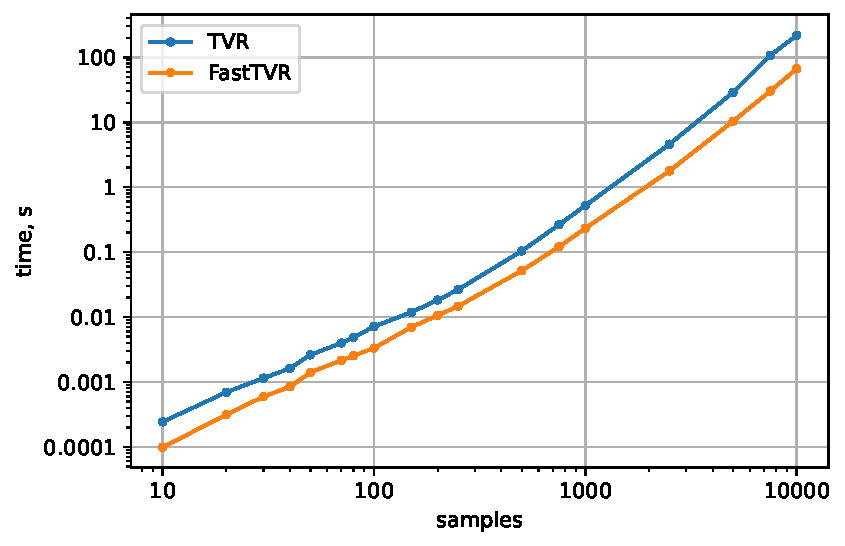
\includegraphics[width=0.9\textwidth]{dif/time}
\caption{Зависимость времени дифференцирования от количества данных}
\label{fig:dif:time}
\end{figure}

    \subsubsection{Анализ алгоритма идентификации}

Для тестирования алгоритма идентификации использовались различные системы ОДУ 1-ого порядка, найденные в книге \cite{synergetics}. Эволюция систем производилась при помощи \texttt{scipy.integrate.solve\_ivp}, в котором используется явный метод Рунге-Кутты четвертого порядка.

Оценка идентифицированной системы производилась при помощи нескольких метрик. В оценке задачи определения значимых членов важно учитывать и те из них, которые не идентифицировались, и те, которые идентифицировались ложно. Поэтому элементарной метрикой может являться само количество таких членов (метрика ME):

\begin{equation}
ME = (FN,\ FP),
\end{equation}

где $FN$ --- false negative --- число потерянных слагаемых,\par
$FP$ --- false positive --- число ложно определенных слагаемых.

Однако такая метрика может быть не очень удобной, и в качестве метрики, объединяющей эти два числа, выбрана IoU --- intersection over union, также известная как коэффициент Жаккара. Эта метрика показывает какая часть из всех фигурирующих слагаемых (предсказанных и истинных) определена верно:

\begin{equation}
J = \frac{TP}{TP + FP + FN},
\end{equation}

где $TP$ --- true positive --- число верно определенных слагаемых.

После выбора метрик, методы регрессии были протестированы снова, на этот раз применительно к задаче идентификации. Так, выяснилось, что алгоритм Lasso плохо для этого подходит. Если простые системы, например, простейшую систему линейных уравнений~(\ref{eq:linear}), еще получается идентифицировать нормально, как это показано на рисунке~\ref{fig:linear:lasso}. Пример конкретной восстановленной системы изображен на рисунке~\ref{fig:linear:lasso_example}.

\begin{equation}
\normalspacing
\begin{aligned}
\dot{x} &= -0.1 x + 2 y \\
\dot{y} &= -2 x - 0.1 y
\end{aligned}
\label{eq:linear}
\end{equation}

\begin{figure}
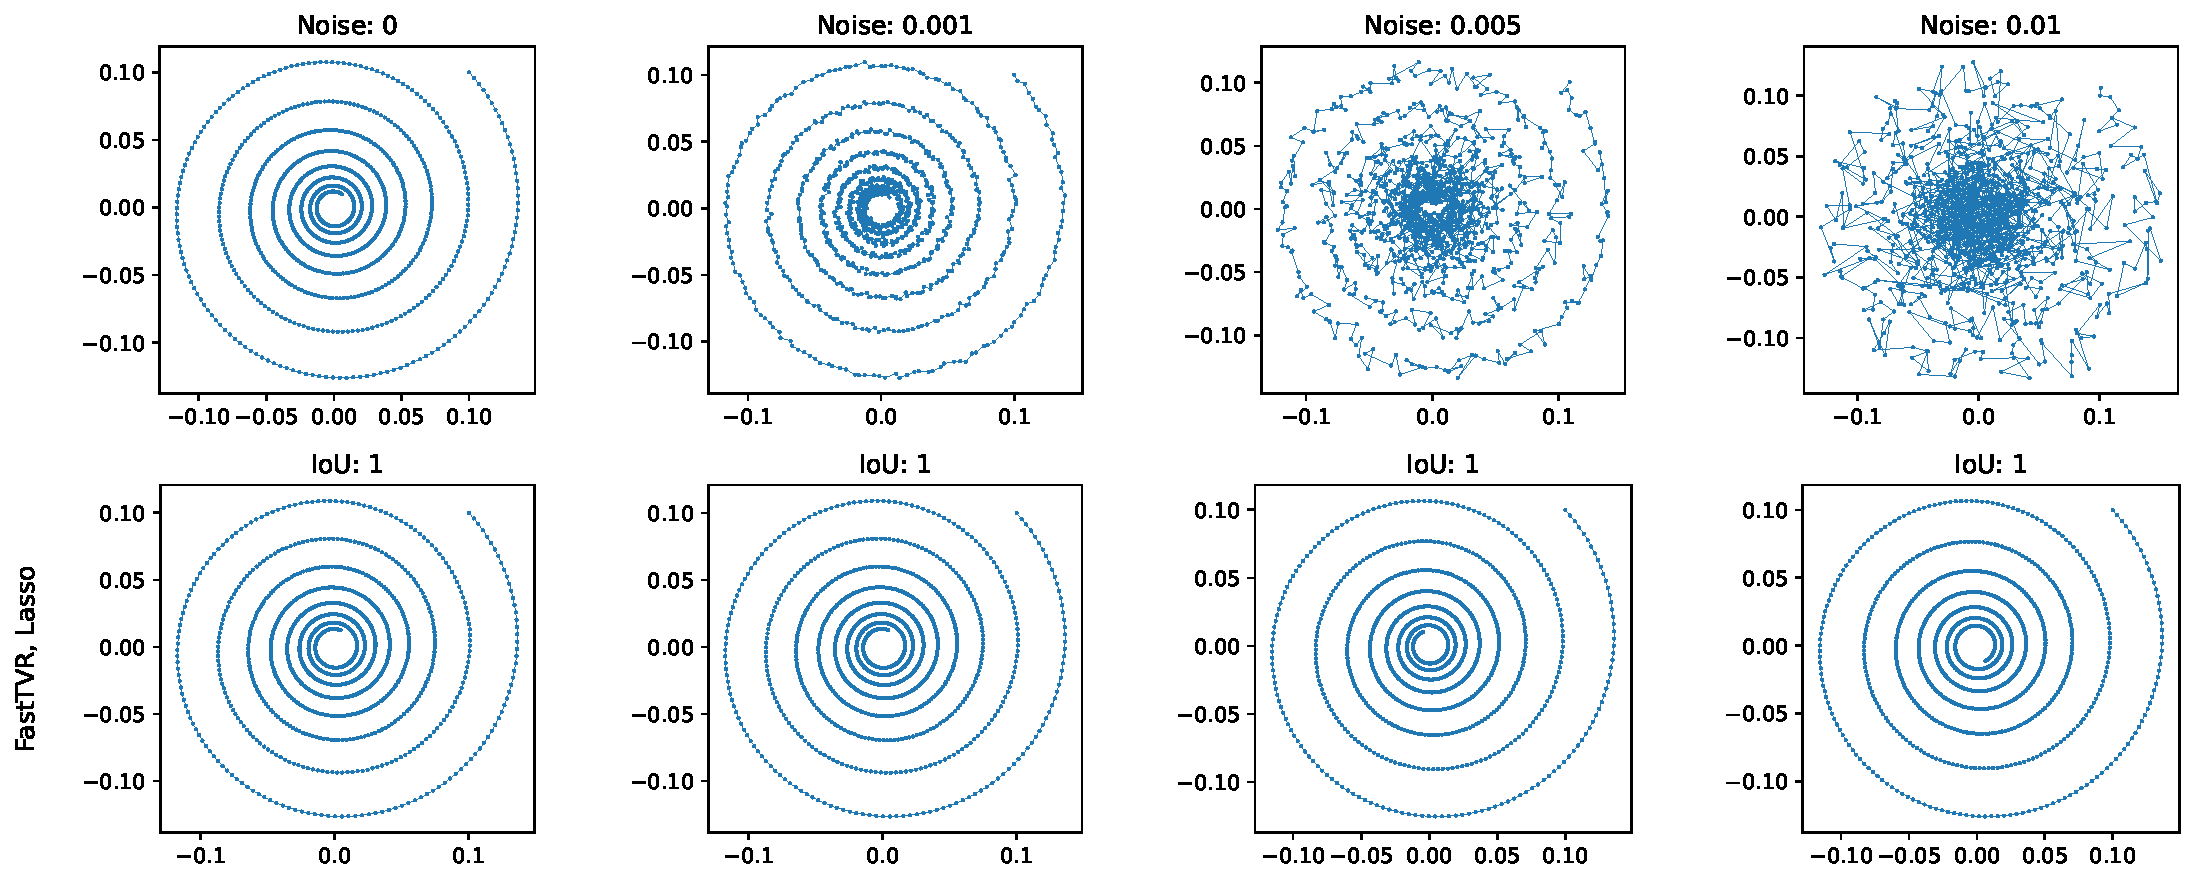
\includegraphics[width=\textwidth]{sindy/linear_lasso}
\caption{Идентификация системы линейных уравнений}
\label{fig:linear:lasso}
\end{figure}

\begin{figure}
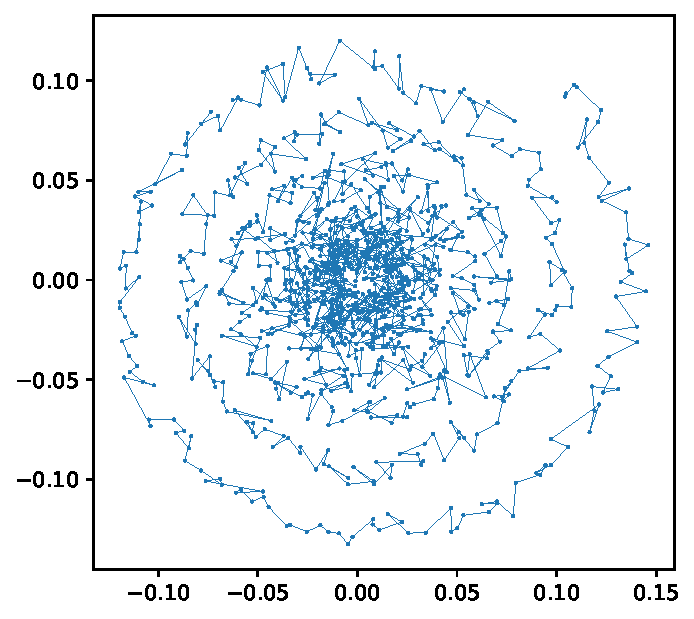
\includegraphics[height=0.28\textheight]{sindy/linear_lasso_orig}\hfill
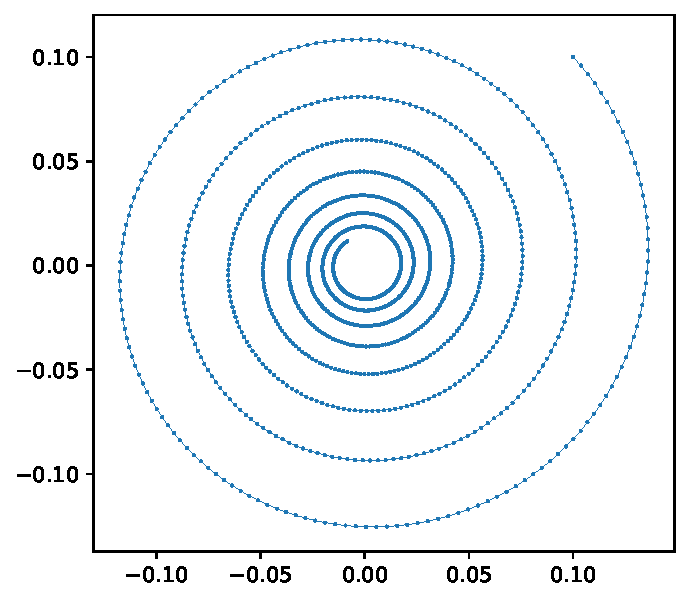
\includegraphics[height=0.28\textheight]{sindy/linear_lasso_res}
\caption{Исходные данные (уровень шума $0.005$) и график восстановленной системы уравнений~(\ref{eq:linear_lasso})}
\label{fig:linear:lasso_example}
\end{figure}

\begin{equation}
\normalspacing
\begin{aligned}
\dot{x} &= -0.115 x + 1.97 y \\
\dot{y} &= -1.94 x - 0.062 y
\end{aligned}
\label{eq:linear_lasso}
\end{equation}

То с более сложными системами возникают проблемы. Это видно на рисунке~\ref{fig:lorenz:lasso}, на котором изображена попытка подбора параметра --- коэффициента регуляризации --- для системы Лоренца. График показывает значения метрики IoU в зависимости от уровня шума и величины параметра, серые пунктирные линии ограничивают область с наибольшим IoU.

\begin{figure}
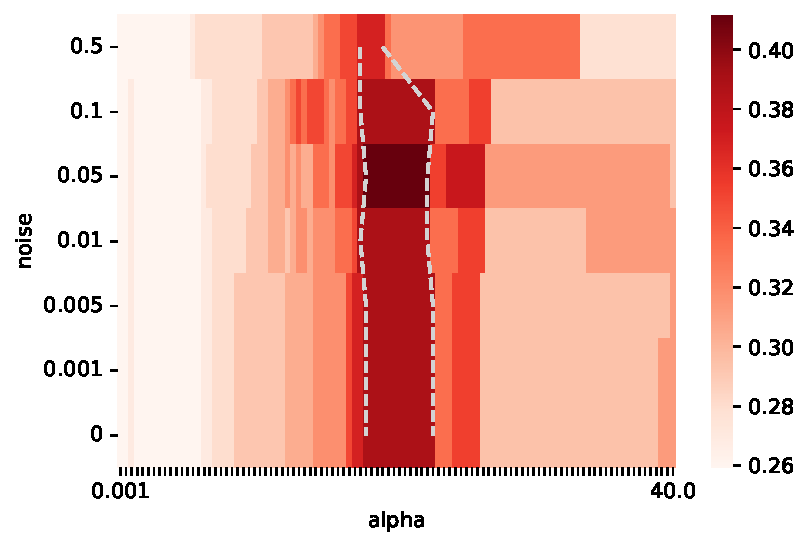
\includegraphics[width=0.9\textwidth]{sindy/lorenz_lasso}
\caption{Подбор параметра $\alpha$ для системы Лоренца}
\label{fig:lorenz:lasso}
\end{figure}

Пример крайне неудачной идентификации показан на рисунке~\ref{fig:lorenz:lasso_example}.

\begin{figure}
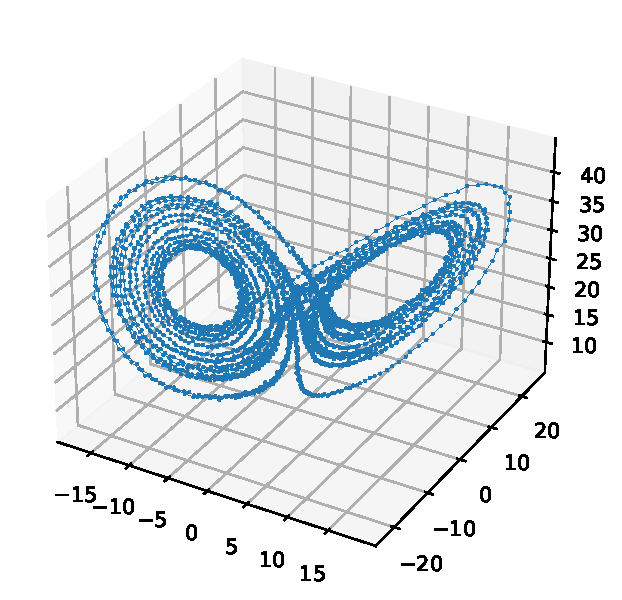
\includegraphics[width=0.49\textwidth]{sindy/lorenz_lasso_orig}\hfill
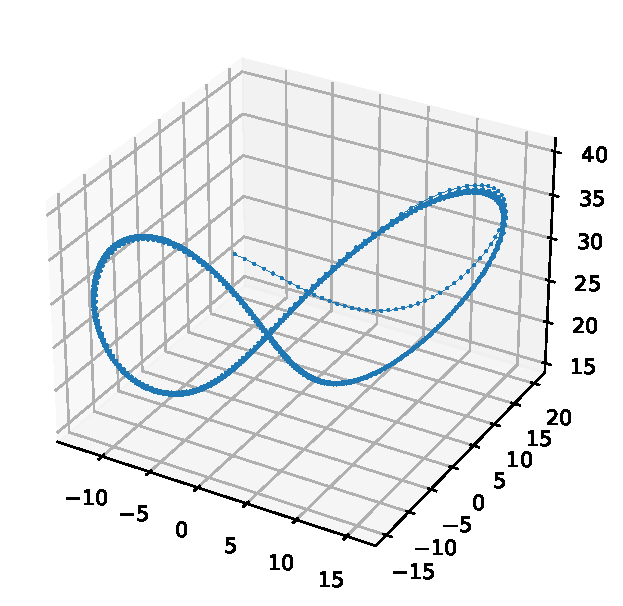
\includegraphics[width=0.49\textwidth]{sindy/lorenz_lasso_res}
\caption{Исходные данные (уровень шума $0.1$) и график восстановленной системы уравнений~(\ref{eq:lorenz_lasso})}
\label{fig:lorenz:lasso_example}
\end{figure}

\begin{equation}
\normalspacing
\begin{aligned}
\dot{x} &= 1.2 y - 0.3 x z + \num{5.1e-4} y^2 + 0.28 y z + 0.0013 z^2 \\
\dot{y} &= 0.47 x + 12 y + 0.0026 x^2 - 0.26 x z - 0.32 y z - 0.004 z^2 \\
\dot{z} &= -0.72 z + 0.57 x^2 + 0.57 x y + \num{9e-5} x z + 0.035 y^2 - 0.088 z^2 \\
\end{aligned}
\label{eq:lorenz_lasso}
\end{equation}

В связи с этим, далее алгоритм Lasso не используется, и в качестве метода регрессии рассматривается только STLSQ.

\paragraph{Система Лоренца}

Систему линейных уравнений решено пропустить из-за ее излишней простоты. Поэтому переходим к аттрактору Лоренца --- решению системы Лоренца (\ref{eq:lorenz}) с начальными значениями $x_0 = 8$, $y_0 = 7$, $z_0 = 27$ и в диапазоне $t \in [0, 20]$. Аттрактор изображен на рисунке~\ref{fig:lorenz}.

\begin{equation}
\normalspacing
\begin{aligned}
\dot{x} &= 10 (y - x) \\
\dot{y} &= x (28 - z) - y \\
\dot{z} &= x y - 8/3 z
\end{aligned}
\label{eq:lorenz}
\end{equation}

\begin{figure}
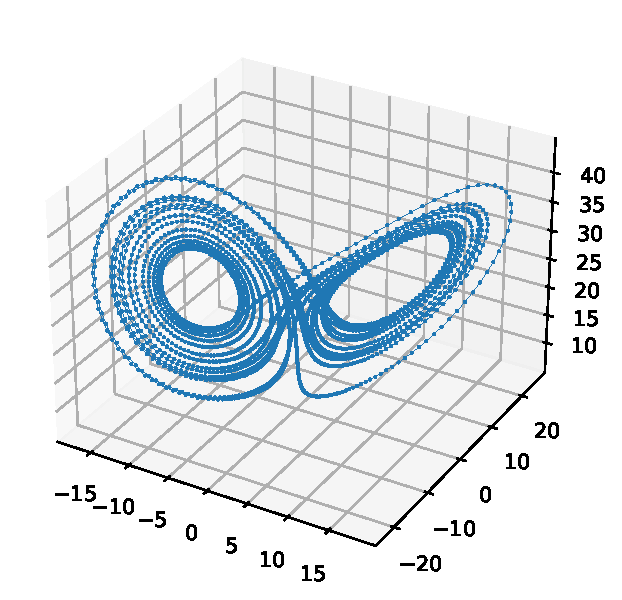
\includegraphics[width=0.5\textwidth]{sindy/lorenz}
\caption{Аттрактор Лоренца}
\label{fig:lorenz}
\end{figure}

Протестируем алгоритм STLSQ. Результаты тестирования изображены на рисунке~\ref{fig:lorenz:stlsq}. Здесь уже наблюдается диапазон значений параметра, при которых достигается приемлемый результат.

\begin{figure}
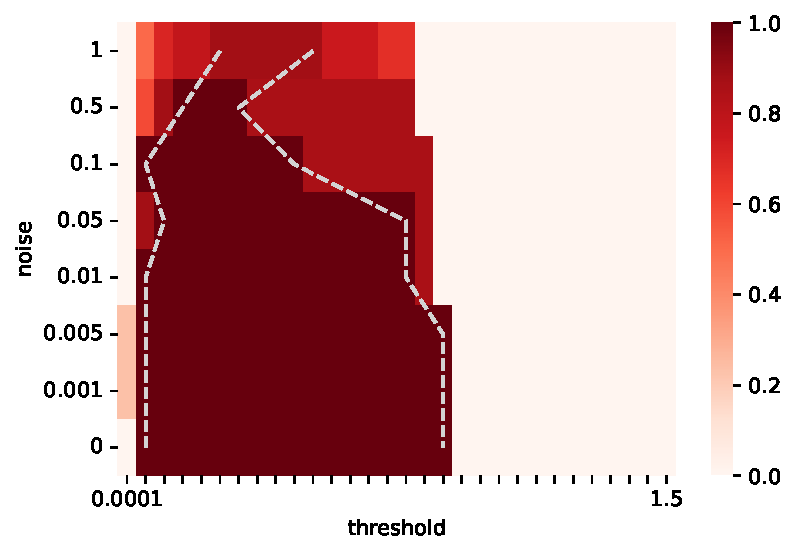
\includegraphics[width=0.49\textwidth]{sindy/lorenz_stlsq_fast_tvr}\hfill
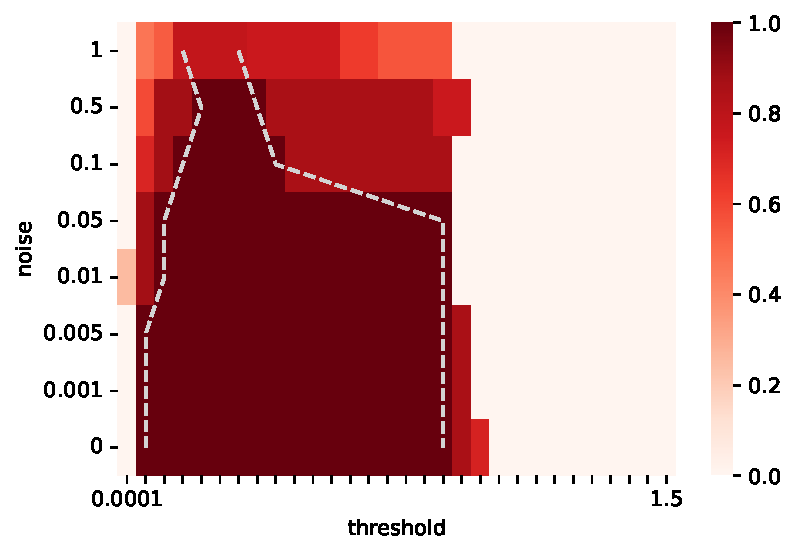
\includegraphics[width=0.49\textwidth]{sindy/lorenz_stlsq_tvr}
\caption{Тестирование алгоритма STLSQ для обоих методов дифференцирования}
\label{fig:lorenz:stlsq}
\end{figure}

Таким образом, имеется возможность подобрать параметры для идентификации системы. На рисунке~\ref{fig:lorenz:test} показаны результаты идентификации вместе со значениями метрики IoU, каждый столбец соответствует одному уровню шума, на первой строке показаны исходные данные.

\begin{figure}
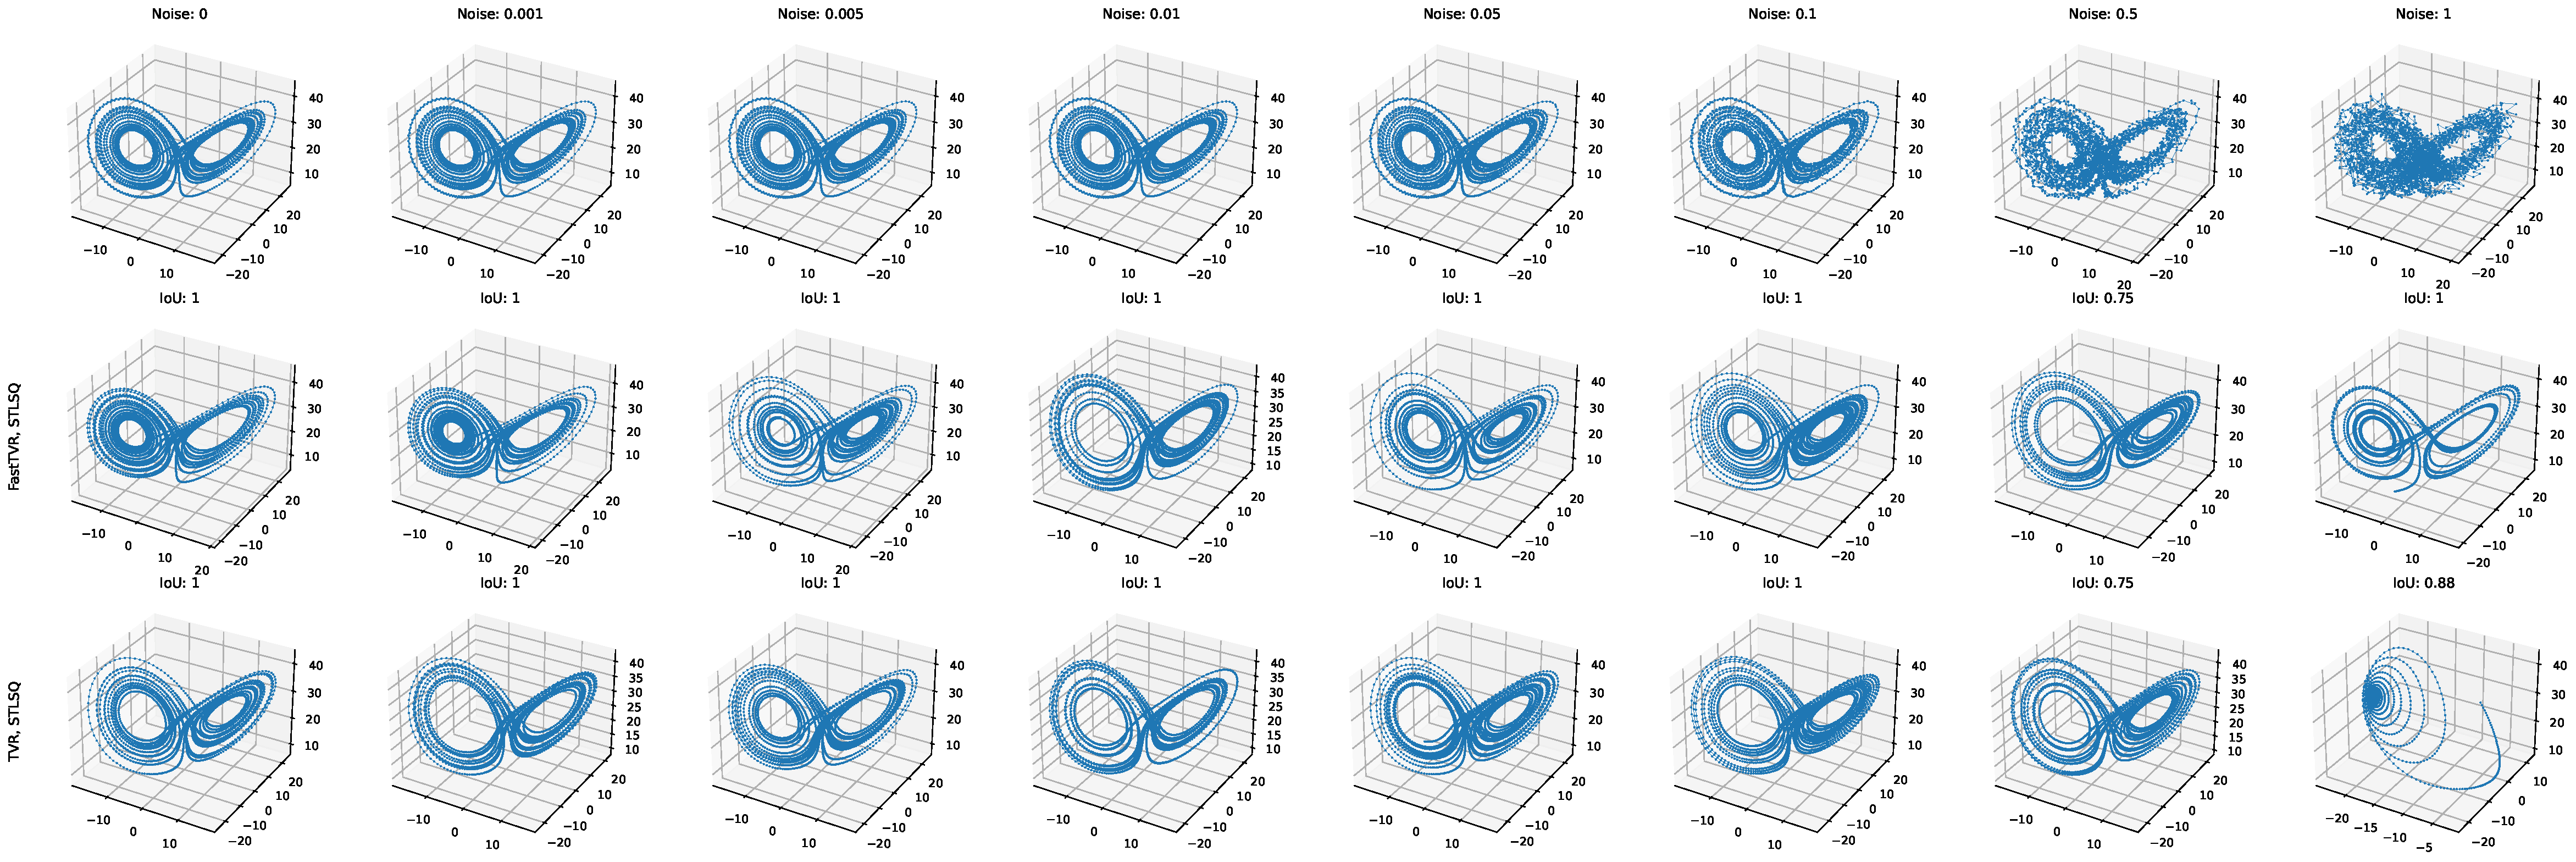
\includegraphics[width=\textwidth]{sindy/lorenz_test}
\caption{Графики восстановленных систем Лоренца}
\label{fig:lorenz:test}
\end{figure}

Можно заметить, что восстановленные системы отличаются от оригинальной. Это связано с тем, что параметры системы восстанавливаются не очень точно. Восстановленные системы уравнений при использовании TVR и уровнях шума $0$, $0.005$, $0.05$, $0.1$, $0.5$ и $1$ имеют следующий вид:

\begin{equation}
\normalspacing
\begin{aligned}
\dot{x} &= -10 x + 10 y                  &\dot{x} &= -9.974 x + 9.979 y \\
\dot{y} &= 27.79 x - 0.917 y - 0.993 x z \qquad &\dot{y} &= 27.78 x - 0.919 y - 0.993 x z \\
\dot{z} &= -2.67 z + 0.999 x y           &\dot{z} &= -2.667 z + 0.999 x y \\
\\
\dot{x} &= -9.97 x + 9.978 y             &\dot{x} &= -9.91 x + 9.928 y \\
\dot{y} &= 27.63 x - 0.861 y - 0.989 x z &\dot{y} &= 27.34 x - 0.833 y - 0.982 x z \\
\dot{z} &= -2.668 z + 0.999 x y          &\dot{z} &= -2.647 z + 0.989 x y \\
\\
\dot{x} &= -9.605 x + 9.683 y        &\dot{x} &= 2.741 - 0.438 x + 4.448 y \\
\dot{y} &= 25.55 x - 0.939 x z       &\dot{y} &= 23.03 x + 0.327 y - 0.877 x z \\
\dot{z} &= 1.2 - 2.658 z + 0.977 x y &\dot{z} &= -2.541 z + 0.955 x y
\end{aligned}
\end{equation}

На рисунке~\ref{fig:lorenz:scores} показаны изменения метрик при использовании TVR: средней ошибки между значениями величин, метрик ME и IoU.

\begin{figure}
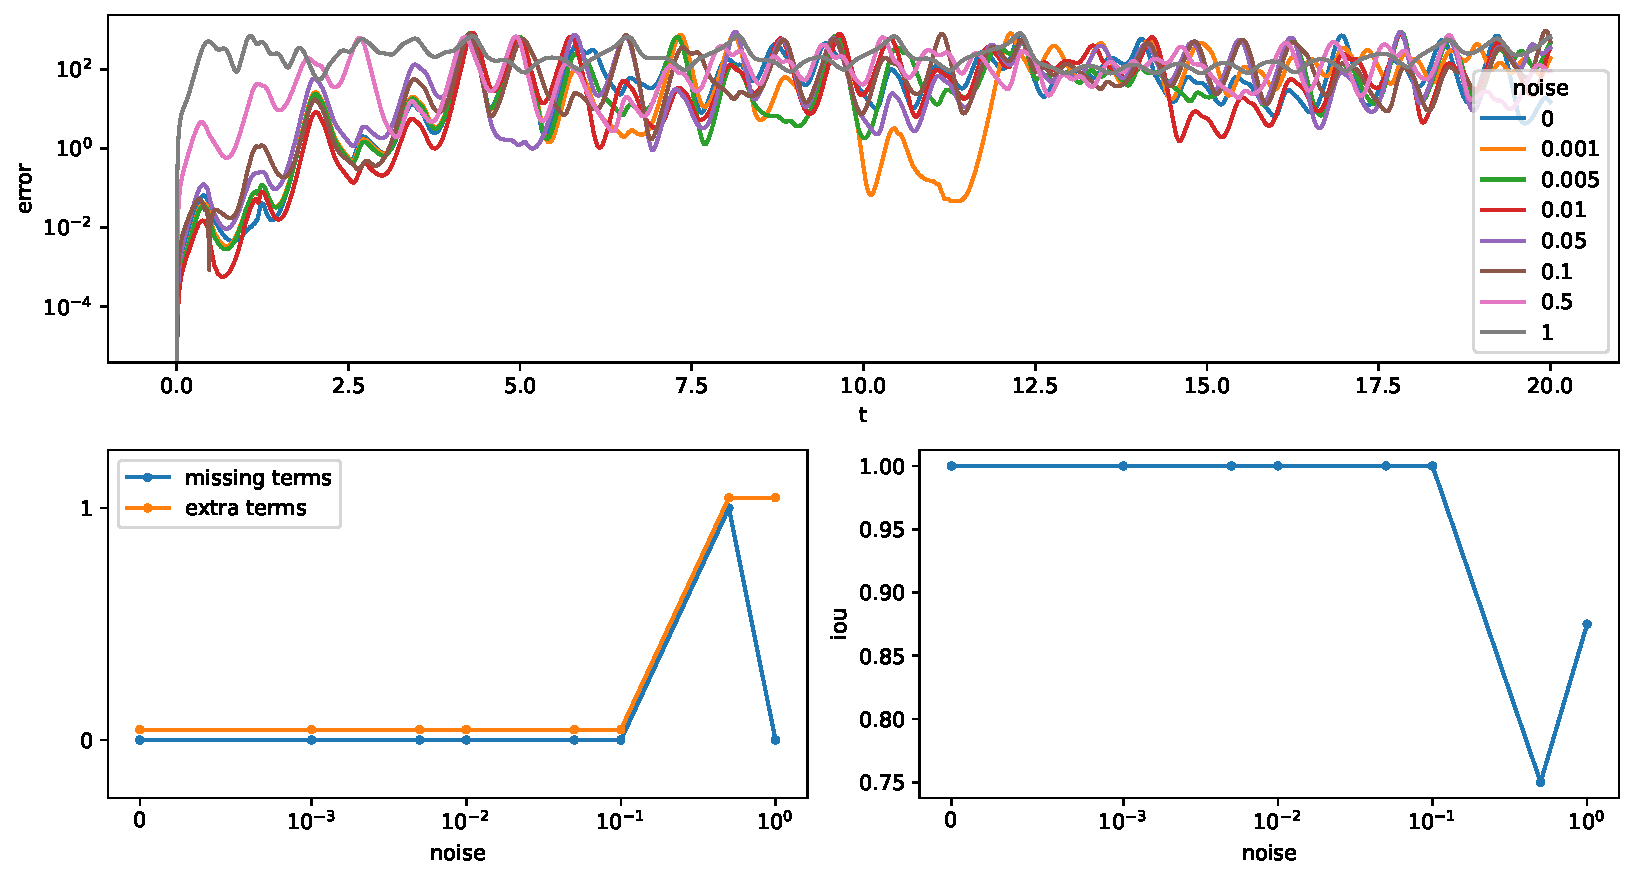
\includegraphics[width=\textwidth]{sindy/lorenz_scores}
\caption{Графики изменения метрик}
\label{fig:lorenz:scores}
\end{figure}

Видно, что, из-за неточных параметров, сравнивать восстановленную систему с исходной напрямую не имеет смысла. Значения средней ошибки получаются большими и примерно одинаковыми для всех случаев. Остальные графики более осмысленные, видно, что число лишних или потерянных слагаемых растет очень незначительно.

\paragraph{Система Мура-Шпигеля}

Система Мура-Шпигеля~(\ref{eq:moore_spiegel}) взята с начальными значениями $x_0 = 0.1$, $y_0 = 0.2$, $z_0 = 0.3$ и в диапазоне $t \in [600, 900]$. Решение системы изображено на рисунке~\ref{fig:moore_spiegel}.

\begin{equation}
\normalspacing
\begin{aligned}
\dot{x} &= y \\
\dot{y} &= z - 0.2 x \\
\dot{z} &= -z / 50 + y (1 - 0.8 x^2)
\end{aligned}
\label{eq:moore_spiegel}
\end{equation}

\begin{figure}
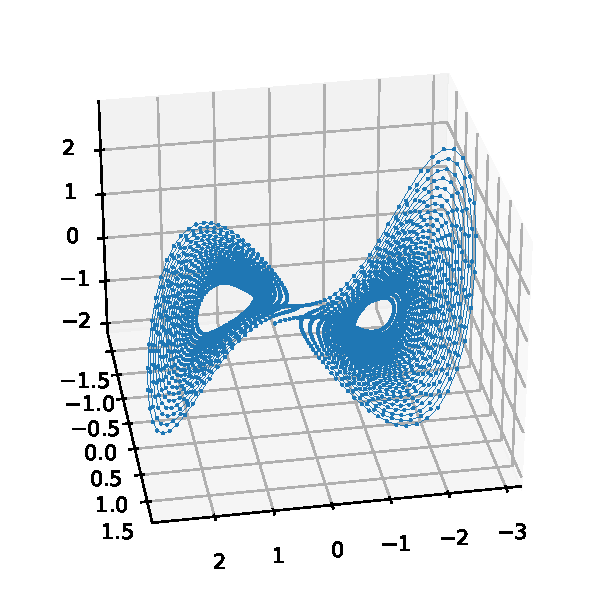
\includegraphics[width=0.5\textwidth]{sindy/moore_spiegel}
\caption{Система Мура-Шпигеля}
\label{fig:moore_spiegel}
\end{figure}

Эту систему было значительно сложнее идентифицировать, как можно видеть из рисунка~\ref{fig:moore_spiegel:test}.

\begin{figure}
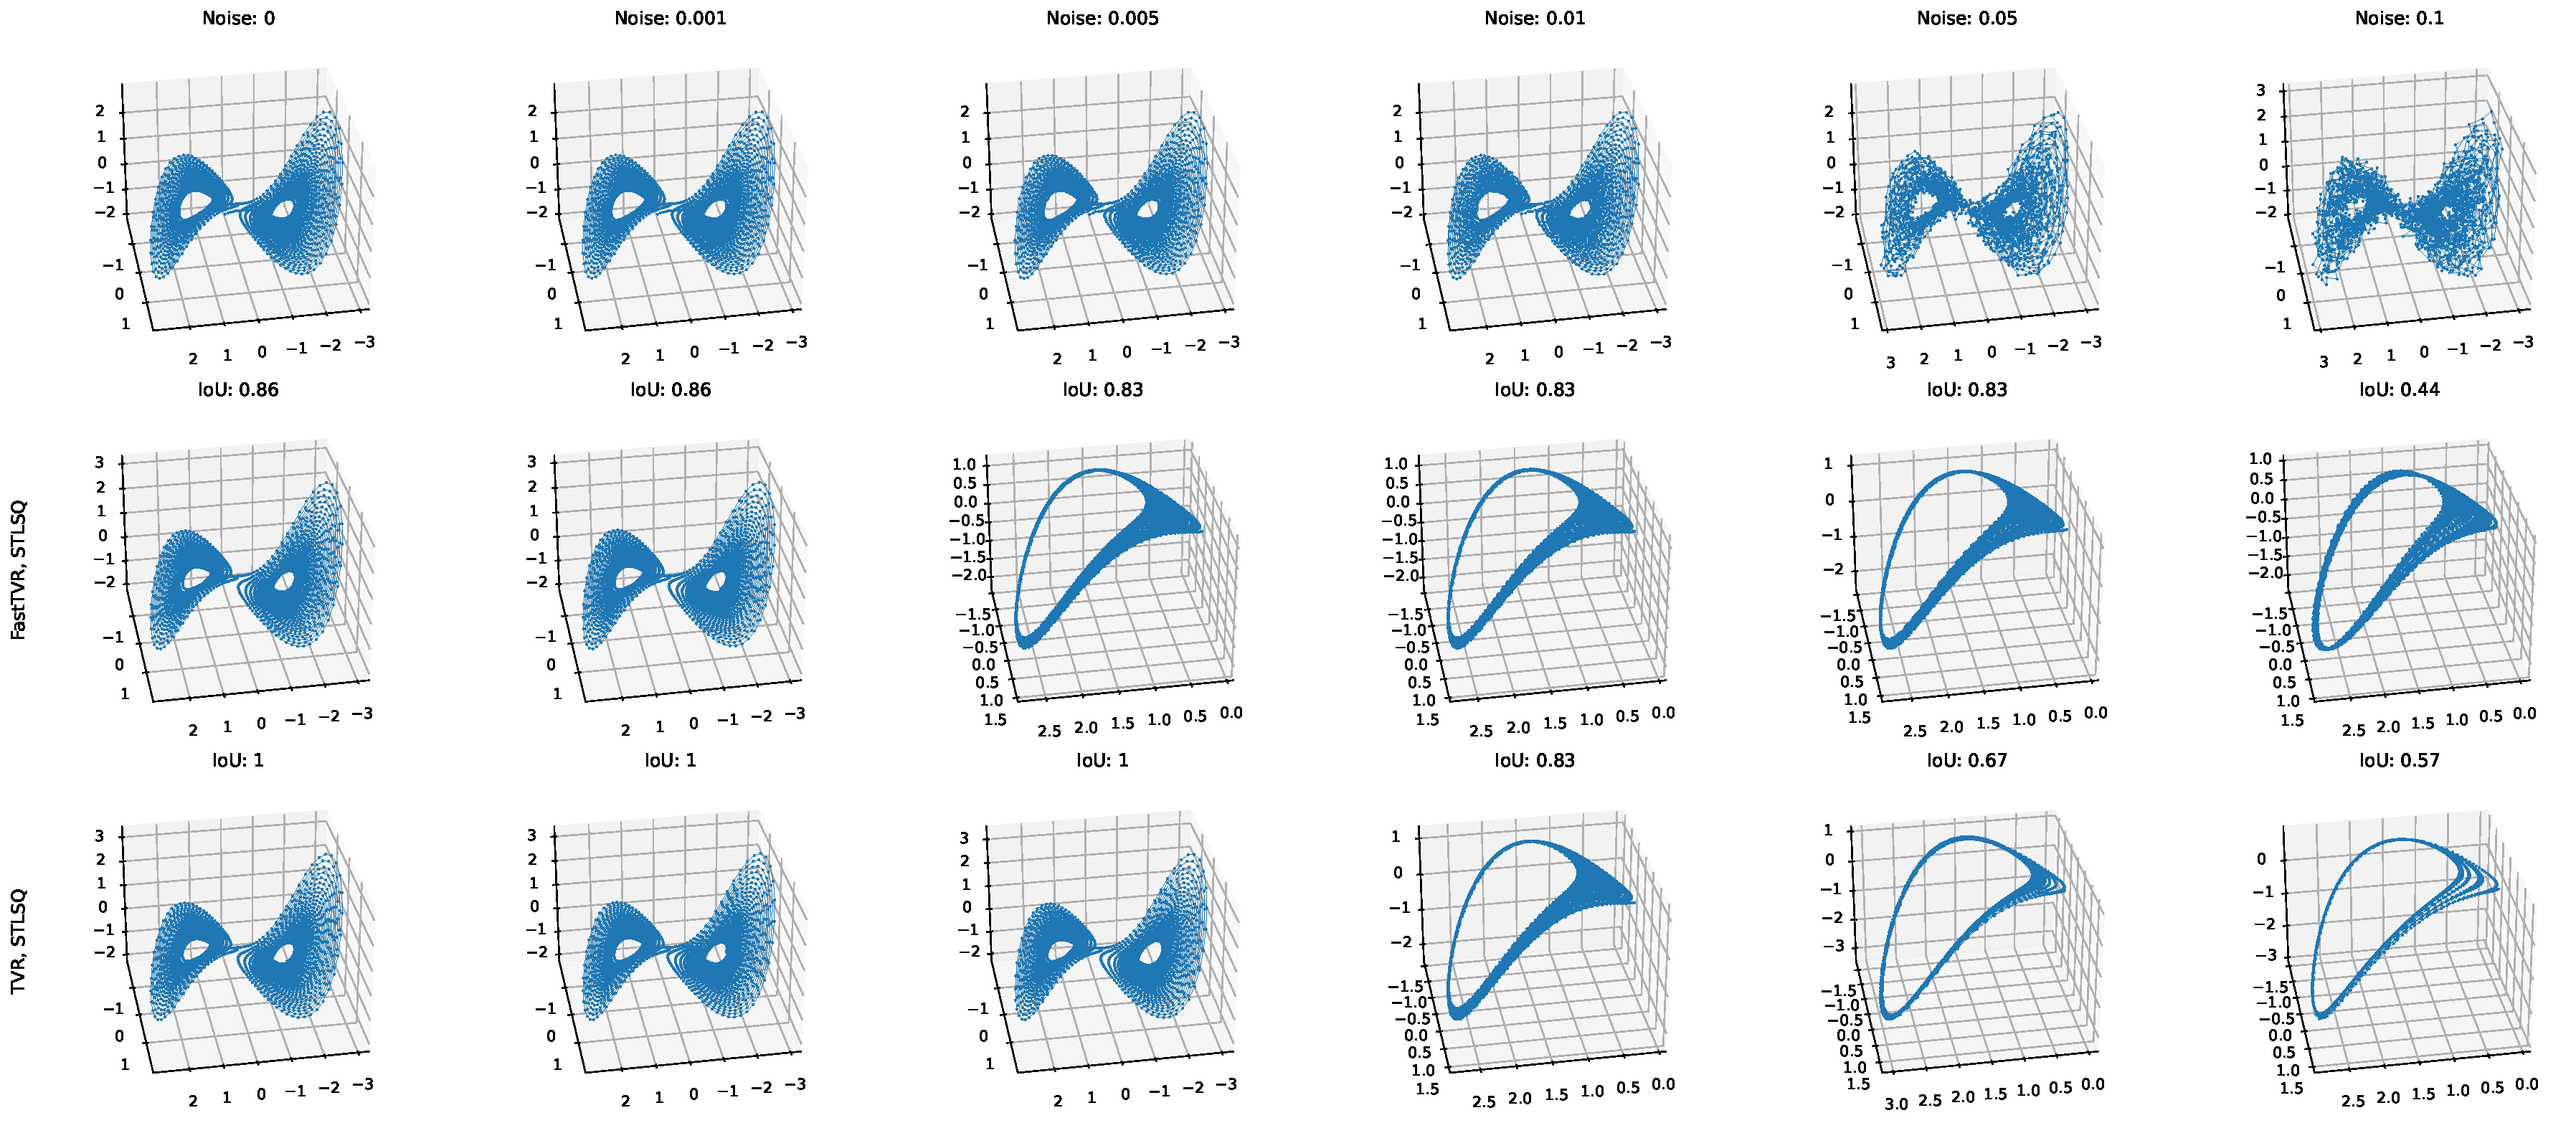
\includegraphics[width=\textwidth]{sindy/moore_spiegel_test}
\caption{Графики восстановленных систем Мура-Шпигеля}
\label{fig:moore_spiegel:test}
\end{figure}

Графики изменения метрик для обоих методов дифференцирования показаны на рисунке~\ref{fig:moore_spiegel:scores}.

\begin{figure}
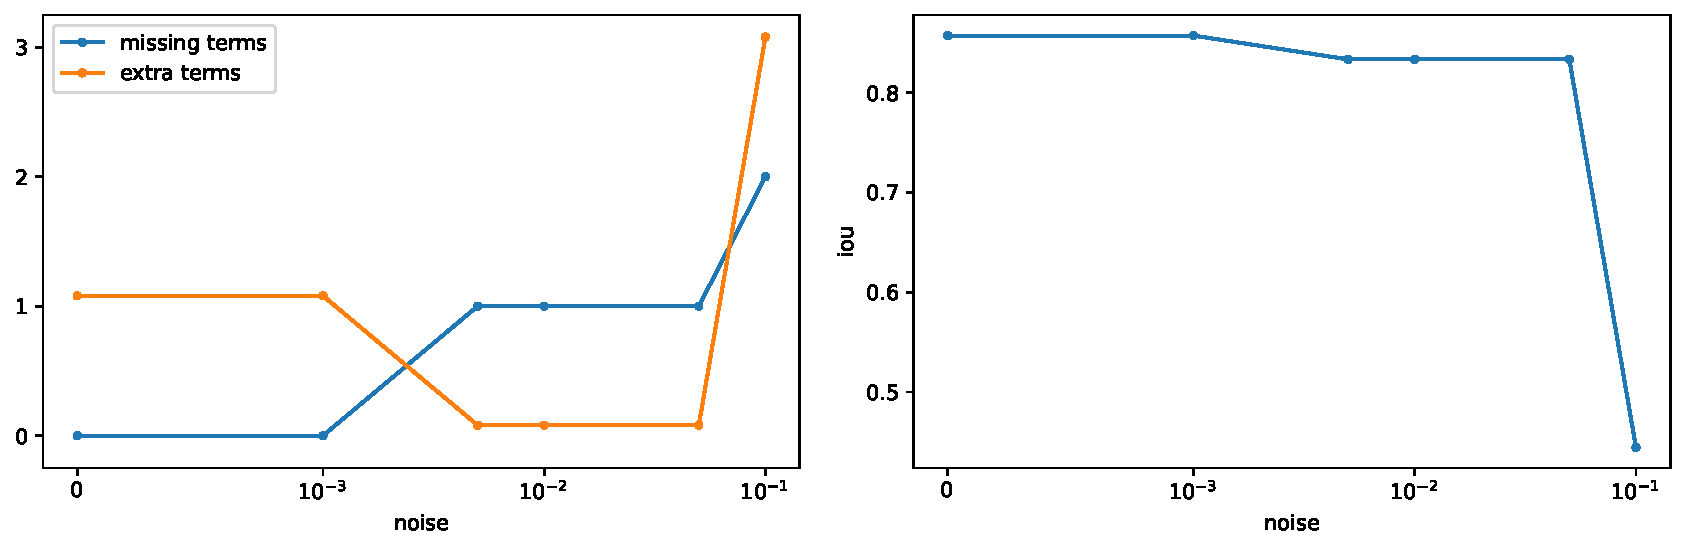
\includegraphics[width=\textwidth]{sindy/moore_spiegel_scores_fast_tvr}
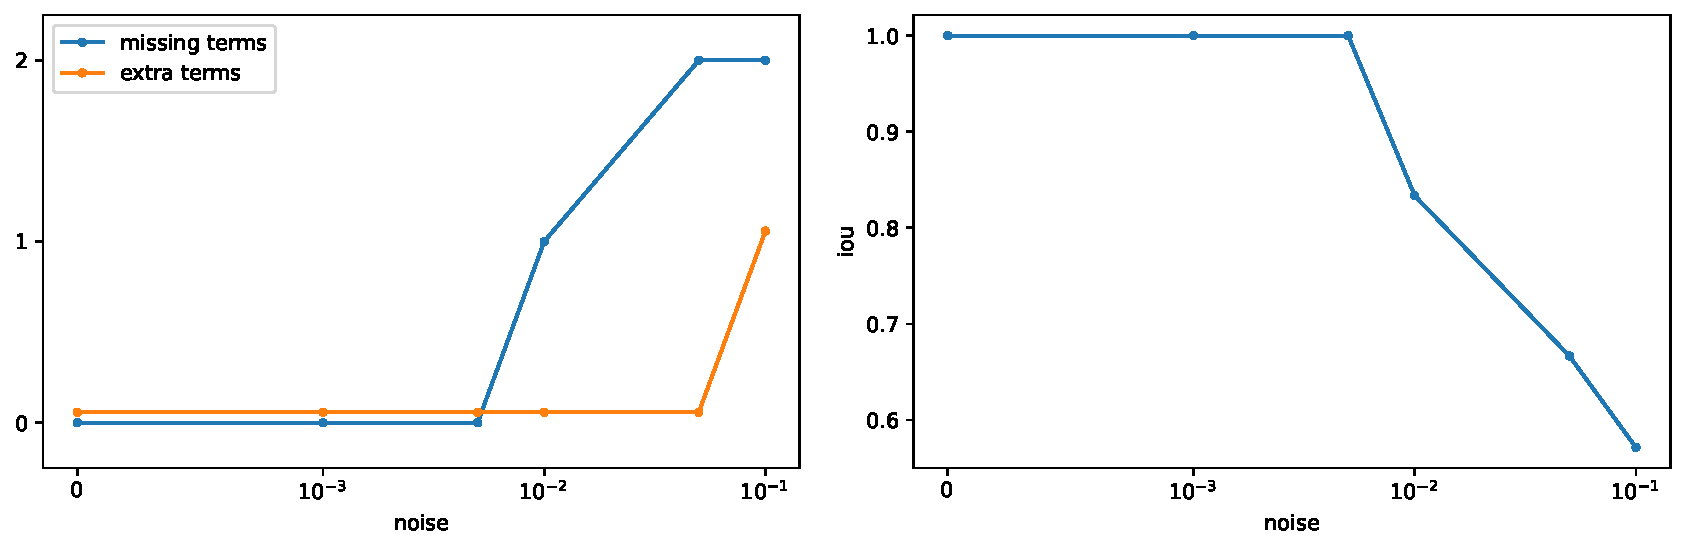
\includegraphics[width=\textwidth]{sindy/moore_spiegel_scores_tvr}
\caption{Графики изменения метрик}
\label{fig:moore_spiegel:scores}
\end{figure}

Ниже приведены восстановленные системы уравнений при использовании TVR, видно, как, начиная с четвертого уровня шума, уравнения теряют слагаемые:

\begin{equation}
\normalspacing
\begin{aligned}
\dot{x} &= 0.977 y                         &\dot{x} &= 0.977 y \\
\dot{y} &= -0.186 x + 0.975 z              &\dot{y} &= -0.186 x + 0.976 z \\
\dot{z} &= 0.992 y - 0.021 z - 0.798 x^2 y \qquad &\dot{z} &= 0.993 y - 0.021 z - 0.799 x^2 y \\
\\
\dot{x} &= 0.984 y                         &\dot{x} &= 0.982 y \\
\dot{y} &= -0.185 x + 0.978 z              &\dot{y} &= -0.187 x + 0.979 z \\
\dot{z} &= 1.006 y - 0.021 z - 0.802 x^2 y &\dot{z} &= 1.046 y - 0.81 x^2 y \\
\\
\dot{x} &= 0.963 y             &\dot{x} &= 0.905 y \\
\dot{y} &= 0.948 z             &\dot{y} &= 0.917 z \\
\dot{z} &= 0.9 y - 0.729 x^2 y &\dot{z} &= 0.757 y - 0.642 x^2 y - 0.167 y z^2
\end{aligned}
\end{equation}
    \subsection{Перспективы дальнейшего развития алгоритма}

В данной работе задача идентификации ограничивается только системами ОДУ 1-ого порядка. Однако возможности алгоритма позволяют делать гораздо больше этого.

Рассмотрим описанный базовый алгоритм. Имея методы обычного численного дифференцирования первого порядка, можно довольно легко получить методы дифференцирования высоких порядков, равно как и методы получения частных производных. Это позволяет производить идентификацию дифференциальных уравнений в частных производных \cite{sindy}, что довольно сильно расширяет область задач, к которым применим данный алгоритм. Также можно отказаться от производных вообще и идентифицировать системы рекуррентных соотношений \cite{sindy} вида:

\begin{equation}
\textsc{x}_{k+1} = f(\textsc{x}_k).
\end{equation}

Кроме этого, можно расширять сам алгоритм идентификации для решения других классов задач. Например, задач теории управления, в частности управления с прогнозирующими моделями (model predictive control) \cite{sindyc_1, sindyc_2}. Такая модификация позволяет идентифицировать системы, в случае ОДУ, вида:

\begin{equation}
\dot{\textsc{x}} = f(\textsc{x}, u),
\end{equation}

где $u$ --- управляющий сигнал.

Или, вместо задачи Коши, идентифицировать системы уравнений краевой задачи \cite{sindy-bvp}. Или все ту же задачу Коши, но для уравнений в неявном виде \cite{sindy-pi} (для таких задач процесс разреженной регрессии еще и крайне хорошо распараллеливается):

\begin{equation}
f(\textsc{x}, \dot{\textsc{x}}) = 0.
\end{equation}

Однако также можно улучшать сам алгоритм. Например, использовать идею ансамблей и обучать несколько моделей вместо одной \cite{sindy-ensemble}. При этом каждая из моделей обучается на подмножестве исходных данных (бутстрэппинг) и идентифицированные системы агрегируются в одну итоговую.

Что касается отдельных частей алгоритма, помимо использования специализированных методов дифференцирования можно пытаться фильтровать сами данные, например, при помощи нейросетевого подхода \cite{nn_denoise}, который отделяет шумовую компоненту, что позволяет работать с шумом любого распределения и даже это распределение идентифицировать.

    
    \conclusion

В ходе выполнения выпускной квалификационной работы бакалавра был реализован алгоритм идентификации систем ОДУ на основе данных. Было произведено тестирование алгоритма на известных системах, по результатам которого можно заключить о его работоспособности. Отдельно от алгоритма были также протестированы и проанализированы его составные части: алгоритмы дифференцирования и разреженной регрессии.

Большую часть работы заняло численное дифференцирование. Применительно к задаче идентификации методы регуляризации полной вариации ранее не применялись, поэтому реализация, анализ, подбор параметров осуществлялись полностью с нуля. С этой точки зрения, использование этих методов можно считать некоторым развитием данной области.

В ходе анализа методов дифференцирования была обнаружена зависимость между уровнем шума и параметром метода. Поэтому для эффективного противодействия шуму в данных, необходимо оценивать его уровень. Этот вопрос не рассматривался в данной работе, однако, для этого существуют различные методы, например, с использованием спектрального анализа.

Алгоритм разреженной регрессии Lasso, сначала показался вполне работоспособным, однако, при тестировании для задачи идентификации работоспособность не подтвердилась. Таким образом, этот алгоритм отброшен.

Тестирование алгоритма идентификации показало сложность данной задачи, отдельно подсветив тот факт, что алгоритмы регрессии и дифференцирования, хорошо работающие в своей области, не достаточно просто объединить, и такие проблемы, как подбор параметров, приходится решать снова, учитывая специфику задачи. Однако с другой стороны, полученные результаты вселяют уверенность в перспективность данного метода и возможность его успешного использования в практических задачах.

    \printbibliography

    \appendix
    \appendixsection{Исходный код}

Репозиторий с исходным кодом расположен по адресу \url{https://github.com/iktovr/bachelor-diploma}.
Ссылка в формате QR-кода представлена на рисунке~\ref{fig:qr}.

\begin{figure}

\includegraphics[width=0.5\textwidth]{qr-code}
\caption{QR-код со ссылкой на репозиторий}
\label{fig:qr}
\end{figure}

\end{document}
